\documentclass[a4paper,oneside,12pt]{book}

%----------------------------------------------------------------------------------------
%	README!
%   Welcome. It's worth having a read through this file
%   to set up the broad parameters, such as the name of
%   the degree, the school/department, the type of work
%   (dissertation/Final Year Project/report, etc. as well
%   as your own details.
%----------------------------------------------------------------------------------------

%----------------------------------------------------------------------------------------
%	COVER PAGE
%   The cover page is laid out in title/title.tex. You can choose a colour
%   or black and white logo
%----------------------------------------------------------------------------------------

%----------------------------------------------------------------------------------------
%	THESIS INFORMATION
%   Put title, author name, degree, type of work, school, department in here
%   It will be used for the title page and for the embedded PDF information
%----------------------------------------------------------------------------------------

\newcommand{\thesistitle}{Comparing Internet Censorship Between Ireland \& Iraq} % Your thesis title, this is used in the title and abstract
\newcommand{\degree}{B.A.I. Computer Engineering} % Your degree name, this is used in the title page and abstract
\newcommand{\typeofthesis}{Thesis} % dissertation, Final Year Project, report, etc.
\newcommand{\authorname}{Griffin Steinman} % Your name, this is used in the title page and PDF stuff
%% Do not put your Student ID in the document, as TCD will not publish
%% documents that contain both your name and your Student ID.

\newcommand{\keywords}{this, that, more} % Keywords for your thesis
\newcommand{\school}{\href{https://www.tcd.ie/scss/}{School of Computer Science and Statistics}} % Your school's name and URL, this is used in the title page

%% Comment out the next line if you don't want a department to appear
\newcommand{\supervisor}{\href{http://www.scss.tcd.ie/}{Dr. Stephen Farrell}} % Your research group's name and URL, this is used in the title page

\AtBeginDocument{
\hypersetup{pdftitle=\thesistitle} % Set the PDF's title to your title
\hypersetup{pdfauthor=\authorname} % Set the PDF's author to your name
\hypersetup{pdfkeywords=\keywords} % Set the PDF's keywords to your keywords
\hypersetup{pdfsubject=\degree} % Set the PDF's keywords to your keywords
}

%% Language and font encodings
\usepackage[T1]{fontenc} 
\usepackage[utf8]{inputenc}
\usepackage[english]{babel}
\usepackage{lipsum}
\usepackage{ragged2e} %allows for text alignment preferences

\usepackage{booktabs}
\usepackage{float}
\usepackage{verbatim}


%% Bibliographical stuff
\usepackage[round,sort,comma,numbers]{natbib}

%% Document size
% include showframe as an option if you want to see the boxes
\usepackage[a4paper,top=2.56cm,bottom=2.56cm,left=2.56cm,right=2.56cm, head = 16pt]{geometry}
\setlength{\marginparwidth}{2cm}
%% Useful packages
\usepackage{amsmath}
\usepackage[autostyle=true]{csquotes} % Required to generate language-dependent quotes in the bibliography
\usepackage[pdftex]{graphicx}
\usepackage[colorinlistoftodos]{todonotes}
\usepackage[colorlinks=true, allcolors=black]{hyperref}
\usepackage{xcolor}
\usepackage{caption} % if no caption, no colon
%\usepackage{sfmath} %use sans-serif in the maths sections too
\usepackage[parfill]{parskip}    % Begin paragraphs with an empty line rather than an indent
\usepackage{setspace} % to permit one-and-a-half or double spacing
\usepackage{enumerate} % fancy enumerations like (i) (ii) or (a) (b) and suchlike
\usepackage{booktabs} % To thicken table lines
\usepackage{fancyhdr}

%\pagestyle{plain} % Embrace simplicity!

%% The Mechanical engineers require your name and ID on the top of every page.
%% Uncomment the following block if you want your name and ID at the top of
%% (almost) every page.

\pagestyle{fancy}
\fancyhf{} % sets both header and footer to nothing
\renewcommand{\headrulewidth}{0pt}
\cfoot{\thepage}
%\ifdefined\authorid
%\chead{\it \authorname\ (\authorid)}
%\else
%\chead{\it \authorname}
%\fi
%% End of block

%% It is not a requirement of the university that the font should be sans-serif, but
%% the Mechanical engineers require it. Comment out the following line to disable it
%%\renewcommand{\familydefault}{\sfdefault} %use the sans-serif font as default

%% If you're not using sans-serif, consider using Palatino instead of the LaTeX standard
\usepackage{mathpazo} % Use the Palatino font by default if you prefer it to Computer Modern

\renewcommand{\theequation}{\arabic{equation}} %% use continuous equation numbers

%% Format Chapter headings appropriately
\usepackage{titlesec}
\definecolor{tcdblue}{cmyk}{0.94, 0.38, 0, 0.27}
\newcommand{\hsp}{\hspace{20pt}}
\titleformat{\chapter}[hang]{\Huge\bfseries}{\thechapter\hsp\textcolor{tcdblue}{|}\hsp}{0pt}{\Huge\bfseries}

\title{\thesistitle}
\author{\authorname}

\frontmatter
\begin{document}
\begin{titlepage}

\center % Center everything on the page

%% All the text parameters should be taken from the start of the main.tex file.
%% You should only alter stuff here if you want to change the layout

%----------------------------------------------------------------------------------------
%	LOGO SECTION
%----------------------------------------------------------------------------------------
%% Choose one of the following -- a colour or black-and-white logo


\includegraphics{title/Trinity_RGB_transparent_main.png}\\[1cm] 
%
\includegraphics[width=12cm]{title/black-stacked-trinity.jpg}\\[1cm] 
\ifdefined\school
\Large \textsc{\school} \\[1.5cm] % Minor heading such as course title
\ifdefined\department
\large \department\\[1.5cm] % Minor heading such as course title
\fi

%----------------------------------------------------------------------------------------
%	TITLE SECTION
%----------------------------------------------------------------------------------------
\makeatletter
\textsc{{ \huge \bfseries \thesistitle}}\\[1.5cm] % Title of your document
 

%----------------------------------------------------------------------------------------
%	AUTHOR SECTION
%----------------------------------------------------------------------------------------

\ifdefined\authorid
\authorname\\ % Your name
\authorid\\[2cm] % Your Student ID
\else
\textsc{\authorname}\\[2cm] % Your name
\fi

%----------------------------------------------------------------------------------------
%	DATE SECTION
%----------------------------------------------------------------------------------------
\textsc{{\large \supervisor}}\\
\textsc{{\large \today}}\\[2cm] % Date, change the \today to a set date if you want to be precise

\textcolor{red}{Adapted from a template created by Prof. Michael Brady, \\ School of Computer Science, TCD \\(remove line 45, title.tex)}


%----------------------------------------------------------------------------------------
%	TYPE OF THESIS SECTION
%----------------------------------------------------------------------------------------
\vfill

\textsc{\normalsize Submitted in partial fulfilment of the requirements for the degree of \\
\degree}

\vfill % Fill the rest of the page with whitespace

\end{titlepage}
\pagenumbering{roman}
\doublespacing

\section*{Declaration}
I hereby declare that this \typeofthesis\ is entirely my own work and that it has not been submitted as an exercise for a degree at this or any other university.

I have read and I understand the plagiarism provisions in the General Regulations of the University Calendar for the current year, found at \url{http://www.tcd.ie/calendar}.

I have also completed the Online Tutorial on avoiding plagiarism `Ready Steady Write', located at \url{http://tcd-ie.libguides.com/plagiarism/ready-steady-write}.
\vspace{1cm}

Signed:~\rule{5cm}{0.3pt}\hfill Date:~\rule{5cm}{0.3pt}


\newpage
\chapter{Abstract}
A short summary of the problem investigated, the approach taken and the key findings. This should not be more that around 400 words.

The must be on a separate page.


what’s the title for our title
abstract one page
five paragraphs 
area and digital twin
project research questions
two paragraphs how to solve them 
paragraph to implement and evaluate
main findings one paragraphs
expanding the abstract


introduction
literature review 
design implementation
evaluation
conclusion





\newpage
\raggedright %\raggedright turns off justification and hypenation

\section*{\Huge{Acknowledgements}}

A special thank you to my mother and father for supporting me.

A special thank you to Eugene O'Rourke and Mark Linnane for their guidance and advice.

\newpage \tableofcontents
%\newpage \listoffigures
%\newpage \listoftables
%\newpage
%\section*{\Huge{Nomenclature}}
%\begin{tabular}{lp{9cm}l}
%A&Area of the wing&$m^{2}$\\
%B\\
%C& Roman letters first, with capitals\ldots\\
%a&then lower case.\\
%b\\
%c\\
%$\Gamma$&Followed by Greek capitals\ldots\\
%$\alpha$&then lower case greek symbols.\\
%$\beta$\\
%$\epsilon$\\
%TLA&Finally, three letter acronyms and other abbreviations arranged alphabetically\\
%\end{tabular}
%\vspace{2cm}

%If a parameter has a typical unit that is used throughout your report, then it should be included here on the right hand side.

%If you have a very mathematical report, then you may wish to divide the nomenclature list into functions and variables, and then sub- and super-scripts.

%Note that Roman mathematical symbols are typically in a serif font in italics.


\mainmatter
\chapter{Introduction}

\section{Research Motivation}

Since its inception, the Internet has served a vast user base that wishes to communicate with one another and spread information. By design, the Internet is a platform that should provide unfiltered content to users. In many cases this content may otherwise be inaccessible by traditional media outlets such as radio or TV. Originally designed to aid government researchers share information, its open and transparent foundation has since changed. Across the globe, governments and other entities are censoring the internet by network manipulation, legislative pressure or otherwise. This is a global threat to fundamental internet user rights and should be treated as such. It is for these reasons that this area ought to be investigated more thoroughly.

Although censorship of certain content (CSAM, pirated entertainment) is widely considered appropriate, normalising this has far reaching consequences on user privacy and free speech. The importance of establishing a quantitative approach to measuring internet censorship cannot be overstated as users are unaware of invisible content in most cases. As a result, the state has a large influence over what ideas can propagate within its borders. Various open-source and community led projects aimed at addressing this issue. Notable examples include the Tor project, OONI, Tails OS and others. However, it is coming to light that this technology is becoming deprecated. In 2022, German police were able to make an arrest after de anonymising Tor traffic using timing analysis. [1]. This highlights the large dichotomy between what users believe governments are capable of and reality. 



For the above reasons, the increasingly pervasive censorship done by governments and corporations around the world is concerning.  


\subsection{Practical Implications}
\subsection{Awareness \& Transparency}
\subsection{Problem Statement}

\section{Background}
\subsection{Global Internet Censorship}
Experts suggest that censorship on the internet is increasing at an alarming rate. “The majority of countries that censor content do so across all four themes, although the depth of the filtering varies. The study confirms that 40 percent of these 2,046 websites can only be reached by an 
encrypted connection (denoted by the "HTTPS" prefix on a web page, a voluntary upgrade from "HTTP").” [4] It is also clear that more and more countries are viewing this as a necessary solution to the unique problems they have. Whether this is appropriate or not, it is happening, and users should be aware of this. 

Governments have a vested interest in maintaining control over telecommunications industries and public internet use. Whether protecting state secrets, preventing cyber crime piracy or acts of terrorism, insulating from perceived negative influence, aiding in the creation of propaganda or otherwise; a large majority of governments choose to exercise inordinate control over the 
information available to its public.  

As more governments and entities began to engage in this, it became increasingly important to hold them accountable. As a result, the ‘Enemies of the Internet’ list was devised. It contains the governments and entities that actively engage in the repression of online freedoms, in the form of censorship and surveillance. As of 2014, there were 19 governments that fit this criterion but by now this number has likely increased. [5] Traditionally, censorship involved monitoring a handful of media and cutting undesirable content, potentially replacing this with a message more in line with the agenda and norms of the locale. However, with the advent of the internet, this distribution of information became decentralised and thus allowed for more expression and freedom in the content consumed by a user. As a result, censorship has become more difficult to conduct, but potentially easier to get away with. Nowadays, governments leverage points of control, network-level filtering and many other techniques to block undesirable content.

\subsection{User Privacy}
\subsection{Censorship vs. Surveillance}
\subsection{Legislation}
Governments can enforce censorship directly through ISPs, tech companies and social media platforms by creating new legislation or simply mandating content be removed. This is used to deplatform individuals and movements during periods of unrest. This is also done in app stores, shutting down entire platforms that are deemed problematic. 



\section{Project Scope}
\subsection{Project Objectives}
Below is an outline of the objectives completed during the duration of the project:

-   To conduct a literature review to identify and evaluate existing censorship measurement tools with a focus on OONI. 

-   To understand how and why censorship is conducted in these countries and how it can be measured. 

-   To collect data using OONI and other sources for both countries. Use historical datasets as well as rerunning tools for up to date data. 

-   To conduct a comparative analysis between the two countries’ datasets. 

-   To consider ethical implications of the research early so as to ensure compliance. 

-   To set up VMs in Israel in order to establish ground truth. 

-   To present high-level findings about the two countries approach to censoring the 
experience of their internet users, make conclusions about the attitudes and values 
present in each locale based on the data collected. 

-   To understand more about the unique situations of both Ireland and Israel, and how 
censorship is used by the state considering this.

\subsection{Core Research Questions}
\subsection{Data Collection \& Analysis Tools}

\section{Ethical Considerations}
\subsection{GDPR and Data Privacy}
\subsection{Potential Risks}
\chapter{State of the Art}
\section{Censorship Mechanisms \& Circumvention Techniques}



\section{Ireland}

\subsection{Censorship in the Past}

According to a report from the United States Department of State in 2011, it was found that there were no government restrictions on access to the internet or that the government actively monitored email or internet chatrooms \cite{stateTechnicalDifficulties}.

The Irish government engages in censoring or blocking the distribution of pirated copryrighted material. In 2009, the Irish Telecom Company, EIRCOM, blocked its customers from accessing the website \textit{The Pirate Bay}. The Pirate Bay is a Swedish website which provides links to copyrighted material. The website was hit with a lawsuit from major record labels and many ISPs around the world agreed to block access to the website as part of the settlement. However, not all Irish ISPs complied. The cable TV operator UPC announced that it would not comply \cite{irishtimesEircomBlock}. 

In alignment with international agreements, the Irish Government blocks access to websites that contain illegal content, such as Child Sexual Abuse Material (CSAM). The government has setup a hotline that allows citizens to anonymously report websites that they suspect contain illegal content, called hotline.ie \cite{hotlineAboutx2013}.

In contrast to other EU countries, Ireland does not have a broad government-mandated filtering system. They instead have the power through the Irish courts to mandate Irish ISPs to block certain websites. In addition, Irish ISPs may voluntarily enforce content filtering and website blocking in alignment with Irish content law.

Up until 2014, Ireland and other EU countries followed data retention laws, which required ISPs to store metadata for law enforcement purposes. In 2014, the European Court of Justice struck down the directive, which led to a change in this law in Ireland \cite{DataRetentionInvalid2014}. After this change, Ireland enacted the \textit{Communications (Retention of Data)(Amendment) Act 2022} \cite{irishlegalDataRetention}. This legislation allows for the general and indiscriminate retention of communications traffic and location data on the grounds of national security, where approved by a judge.

\subsection{Current Censorship}

\section{Iraq}

\section{Tools}

\subsubsection{The Tor Browsers}

\subsection{VPNs}

\chapter{Methodology}

\section{The OONI Probe}

\subsection{Background of OONI}

The Open Observatory of Network Interference (OONI) project was started in 2012 as a non-profit open-source software project aimed at identifying and documenting internet censorship around the world \cite{ooniAbout}. The OONI organization openly publishes measurements and provides a public archive on network interference from across the world. 

\subsection{Data-Collection}

\subsubsection{Web Connectivity Test}

The Web Connectivity test determines if, and how, access to a specific website may be blocked. To do this, OONI Probe performs several checks from the network where the test is run and compares the results with measurements collected from a control network where censorship is not expected. If the measurements differ significantly, censorship techniques are likely used on the local network. This test is designed to perform the four different actions: Resolver Identification, DNS Lookup, TCP Connect, HTTP GET Request.

The Web Connectivity test begins by identifying the DNS resolver in use on the network. It achieves this by sending DNS queries to special domains, which disclose the resolver’s IP address. Once the resolver is identified, the test performs DNS lookups to determine which IP addresses (and potentially other host names) are mapped to the tested domain. After collecting that information, the test attempts to establish a TCP session on port 80 or port 443, depending on whether the URL uses HTTP or HTTPS. Finally, once the TCP connection is successful, the test sends an HTTP GET request to the server hosting the website; under normal circumstances, the server will respond with the requested webpage content \cite{ooniConnectivityTest}.

\subsubsection{Circumvention Test}

The circumvention test is used to check weather Psiphon, Tor, or RiseupVPN are blocked on a given network. These are tools used to circumvent censorship by utilizing VPN, SSH, and HTTP proxy technologies. 

The Psiphon VPN serves as a tunnel that enables you to circumvent censorship by connected you to an uncensored portion of the internet \cite{ooniPsiphonTest}. The Psiphon test first uses Psiphon’s own code to establish a Psiphon tunnel. After the tunnel is created, the test attempts to load a webpage to see if Psiphon actually works for accessing the internet. If the tunnel is successfully set up and the webpage loads, Psiphon is functioning on the tested network and can bypass censorship. If the tunnel is established but the webpage does not load, Psiphon is blocked in some way, preventing access to online resources. Finally, if the test cannot even create the Psiphon tunnel, it indicates that Psiphon is completely blocked on that network \cite{PsiphonTestGitHub}.

The Tor Test \cite{TorTestABOUTOONI} automatically checks whether Tor is accessible in a given network by examining the reachability of core components such as Tor directory authorities, OR ports, and obfs4 bridges. It first attempts to retrieve the Tor consensus from directory authorities, then tries to connect to OR ports (including those of directory authorities) via a TLS handshake, and finally tests obfs4 bridges through an obfuscated handshake. If all of these steps succeed, Tor is likely usable in the tested network (unless it is blocked in ways not covered by the test). If any step fails, Tor may be blocked and therefore unavailable on that network \cite{TorTestGitHub}.

The RiseUpVPN test evaluates if the bootstrap servers used during the self-configuration of the VPN clients can be reached. The test also checks if RiseupVPN’s gateways can be reached on different ports and transports \cite{RiseUpVPNTest}. This test was contributed by the LEAP collective \cite{leapLEAPEncryption}.

\subsubsection{Instant Messaging Test}

The Instant Messaging test is used to check weather WhatsApp, Facebook Messenger, Telegram, and Signal are blocked on a given network.

The Whatsapp test attempts to determine is there is any interference or blockage of it's App or Web Interface. To to this, the OONI probe attempts to perform an HTTP GET request TCP Connection, and DNS lookup to WhatsApp's enpoints. These include the endpoints used by the WhatsApp mobile app, the registration service, and the web interface \cite{ooniWhatsAppTest}. To conduct these tests, the OONI probe attempts to open TCP sockets towards WhatsApp endpoints on Ports 443 and 5222. If these connections fail or are rejected, it is seen as an indicator of blockage at the TCP level. The probe then verifies if the DNS resolution returned a valid IP address that is registered to WhatsApp. If the resolved IP address does not belong to WhatsApp, it can indicate DNS level blocking or tampering. And to check if the WhatsApp registration service is working correctly, an HTTP GET request is sent to the URL \url{https://v.whatsapp.net/v2/register}. The request is considered successful if there is no DNS, TCP connect, TLS (Transport Layer Security), or I/O error \cite{WhatsAppTestGitHub}. 

The Facebook Messenger Test is used to examine the reachability of the service within a tested network. The OONI probe begins by attempting to perform a TCP connect and DNS lookup to facebook's endpoints \cite{ooniFacebookMessenger}. The test verifies if Facebook Messenger endpoints resolve to consistently known IPs and if it's possible to establish TCP connections to them on port 443. For each endpoint tested, an A lookup for the domain name is performed and it is considered consistent if the IP is inside of a netblock linked to the \textit{Facebook Authonomous System Number} (AS32934) \cite{FacebookTestGitHub}.

The Telegram Test is used to examine the reachability of Telegram's app and web version within a tested network. The telegram access points (DCs) are those used by the desktop client, and they have six unique IP addresses. The test establishes a TCP connection to all of the access point IP addresses and attempts to send a POST HTTP request to each of them. If all TCP connections on ports 80 and 443 fail, Telegram is considered to be blocked at the TCP level. Otherwise, Telegram is considered to be working as intended \cite{TelegramTestGitHub}. 

The Signal Test is used to measure the reachability of the Signal messaging app within a tested network. The test checks if it is possible to establish a TLS connection and send an HTTP GET request to the Signal server endpoints \cite{ooniSignalTest}. A DNS query to \url{uptime.signal.org} is also performed to check if the backend servers are down \cite{SignalTestGitHub}. 

\subsubsection{Middlebox Test}

A Middlebox is a computer networking device that transforms, filters, and manipulates traffic for purposes other than packet forwarding. These include network address translators, load balancers, and deep packet inspection (DPI) devices. The presence of Middleboxes can lead to evidence of censorship and/or traffic manipulation, but it can also be indicative of a less malicious intent, such as network caching.

The OONI Middlebox test consists of two main operations: HTTP Header Field Manipulation and HTTP Invalid Request Line. The HTTP header field manipulation test emulates an HTTP request towards a server, but sends HTTP headers that have variations in capitalization. These requests are sent to a backend control server which send back any data it receives, and if these requests return exactly as we sent them, it is assumed there is no middlebox present. If the alterations of the headers come back normalized, it can be assumed that there was packet manipulation of some kind, leading to the confirmation of presence of Middleboxes It is worthy to note that false negatives can happen in this test, as some ISPs use highly sophisticated software that can disguise the presence of Middleboxes \cite{ooniHTTPHeader}.  

The HTTP Invalid request line test sends an invalid HTTP request to an echo service listening on the standard HTTP port, rather than a valid one. If the request is returned to the user exactly as it was sent, it can be concluded that there is no evidence of the presence of a Middlebox. However, it is possible that this invalid request can be intercepted by a Middlebox that triggers an error that is sent back to the probe. This is evidence that there is a Middlebox present in the network. It is worthy to note that false negatives are possible as some ISPs use highly sophisticated software that is designed not to trigger such errors \cite{ooniHTTPInvalid}. 

\subsection{Data Collection and Transparency}

All results from OONI Probe tests are automatically sent to OONI's servers and published on the OONI explorer. This transparency ensures that anyone can explore the measurements for themselves. OONI aggregates measurements by country, time, and type of test. It highlights "confirmed" cases of blocking when there is strong enough certainty in the test result, but it also publishes anomalies that might be considered false positives. 

The OONI team also work to release comparative analysis and real-time alerts for significant internet censorship related events. This would include events such as a sudden surge in social media blockage, or a complete drop off of internet traffic in certain areas. The OONI Mesaurement Aggregation Toolkit (MAT) can be used to visualize these events and potentially identify emerging trends. 

\section{Data Collection}

\subsubsection{Ireland}

To collect network data in Ireland, the OONI CLI was installed on a MacBook Air M2 located in Ireland. The OONI probe was installed based on the CLI instructions found on the OONI website \cite{OONISCLI}. The OONI probe by default does not run automatic tests on the Mac version of the CLI, and this was manually enabled during the installation process.

\subsubsection{Iraq}

To collect network data in Iraq, a Virtual Machine was set up using the provider \textit{LightNode} \cite{lightnodeLightNodeGlobal} on a cloud server located in Baghdad. The cloud server was running Linux Ubuntu version ...PUT VERSION HERE...The OONI probe was installed using the CLI instructions available on the OONI website \cite{OONISCLI}. By default, the OONI probe runs censorship tests in the background once per day, and saves that data in a specific directory, as well as publishes the data publicly.

\subsubsection{Overlapping Information}

In addition to these automated tests, manual tests were conducted once per day to collect data. The OONI CLI user guide provided the specific commands to carry out these tests as well as how to run tests on specific files or test sets \cite{ooniUserGuideCLI}. The first and second day of data collection period used the comprehensive OONI test suite, which ran every test available, including 2200 websites. This broad test suite was used to identify blocked websites that could be added to a smaller test set of websites.

Following the initial testing, a set of 127 websites was collected. This test set included blocked websites from the broad OONI test set, some websites from the most known blocked websites worldwide \cite{blocksiteMostBlocked}, the top 50 most visited websites in Ireland \cite{top50irishwebsites}, and the top 50 most visited websites in Iraq \cite{top50IraqWebsites}. This test set was used in both countries for a span of 15 days.

To parse the OONI data, a python script was written that took in the raw bash/cmd output and organized the results of the test into a neatly formatted CSV file. This made data analysis much easier to complete. Each of the four main tests were recorded as raw bash/cmd output and parsed into CSV files for analysis. All results and OONI links are available on this project's public GitHub Repository, which can be found in the appendix of this report.

\section{Challenges \& Limitations}



\chapter{Results and Discussion}

The data and discussion of results below combine data gathered using the OONI probe in Ireland and Iraq with published OONI data from the OONI Measurement Aggregation Toolkit (MAT).

\section{Test Results}

\subsection{Website Accessibility Results}

\subsubsection{Collected Data}

This section analyses website accessibility data collected using the OONI Probe. The tests were carried out locally in Ireland and through a virtual machine (VM) hosted in Iraq. The results reflect the average number of websites blocked daily over a 9-day testing period. The findings are categorized by country, blocking method, and website category to highlight differences in censorship patterns.

\vspace{2em}

\begin{table}[H] 
\centering 
\caption{Proportion of Blocked vs. Unblocked Websites by Country (Daily Average Over 9 Days)} 
\begin{tabular}{lccc} 
\toprule 
\textbf{Country} & \textbf{Unblocked} & \textbf{Blocked} & \textbf{Blocked (\%)} \\
\midrule 
Ireland & 105 & 32 & 23.4\%  \\
Iraq & 108 & 29 & 21.2\% \\
\bottomrule 
\end{tabular} 
\label{tab:blocked_summary} 
\end{table}

It is worth noting that the results in table \ref{tab:blocked_summary} may not be reflective or indicator of the number of blocked websites in each country. The list of websites that yielded these results is comprised of commonly visited websites in each country along with some of the most known commonly blocked websites worldwide. A more in-depth discussion of these results can be found in section \ref{sec:Website-Accessability-Analysis}.

\vspace{2em}

\begin{table}[H] 
\centering 
\caption{Distribution of Detected Blocking Methods by Country} 
\begin{tabular}{lcccc} 
\toprule 
\textbf{Blocking Method} & \shortstack{\textbf{Iraq} \\ \textbf{Frequency}} & \textbf{Iraq \%} & \shortstack{\textbf{Ireland} \\ \textbf{Frequency}} & \textbf{Ireland \%} \\
\midrule 
TCP/IP         & 18 & 60.0\%  & 15 & 55.6\% \\
DNS            & 1  & 3.3\%   & 6  & 22.2\% \\
HTTP           & 3  & 10.0\%  & 1  & 3.7\% \\
Error/Failure  & 8  & 26.7\%  & 5  & 18.5\% \\
\bottomrule 
\end{tabular} 
\label{tab:blocking_methods_comparison} 
\end{table}

TCP/IP blocking emerged as the most common method, indicating low-level network interference. Ireland had more cases of DNS-based blocking than Iraq, whereas HTTP and Error/Failure blocks were more evenly distributed.

\vspace{2em}

\begin{table}[H] 
\centering 
\caption{Number of Blocked Websites by Category and Country} 
\begin{tabular}{lccc} 
\toprule 
\textbf{Category} & \textbf{Total} & \shortstack{\textbf{Ireland} \\ \textbf{Blocked (\%)}} & \shortstack{\textbf{Iraq} \\ \textbf{Blocked (\%)}} \\
\midrule 
Uncategorized                      & 30 & 12 (40.0\%)  & 10 (33.3\%) \\
Piracy / Streaming / File Sharing  & 20 & 10 (50.0\%)  & 4 (20.0\%)  \\
News / Media                       & 20 & 2 (10.0\%)   & 2 (10.0\%)  \\
Adult Content                      & 20 & 0 (0.0\%)    & 0 (0.0\%)   \\
Creative / Educational / Misc      & 15 & 0 (0.0\%)    & 0 (0.0\%)   \\
General / National Services        & 9  & 1 (11.1\%)   & 2 (22.2\%)  \\
Streaming / Social Media           & 9  & 1 (11.1\%)   & 1 (11.1\%)  \\
Religious                          & 4  & 2 (50.0\%)   & 3 (75.0\%)  \\
VoIP / Communication               & 2  & 1 (50.0\%)   & 1 (50.0\%)  \\
Gambling                           & 2  & 2 (100\%)    & 2 (100\%)   \\
Email/Privacy Tools                & 2  & 0 (0.0\%)    & 1 (50.0\%)  \\
Adult / Alcohol                    & 2  & 0 (0.0\%)    & 2 (100\%)   \\
LGBTQ+                             & 1  & 1 (100\%)    & 1 (100\%)   \\
AI / Technology                    & 1  & 0 (0.0\%)    & 0 (0.0\%)   \\
\bottomrule 
\end{tabular} 
\label{tab:category_block} 
\end{table}

The most frequently blocked category in Ireland was “Piracy / Streaming / File Sharing” (50\%), followed closely by “Uncategorized” sites (40\%). In Iraq, “Religious” websites experienced the highest rate of censorship (75\%), with additional blocks targeting sites associated with adult content and gambling.

\subsubsection{Public OONI Data}

This section is an analysis of publicly available OONI data over the previous 30 day period in Ireland and Iraq. The data in table \ref{tab:category_block} is the average over the 30-day period.

\vspace{2em}

\begin{table}[H]
\centering
\caption{Website Blocking based on Public OONI Data}
\begin{tabular}{lcc}
\toprule
\textbf{} & \textbf{Ireland} & \textbf{Iraq} \\
\midrule
Number of Websites Tested           & 1695 & 3703 \\
Number of Successful Connections    & 1628 & 3353 \\
Number of Anomalies                 & 43 & 262 \\
Number of Failures                  & 24 & 88 \\
\bottomrule
Percentage of Total Blocked         & 2.5\% & 7\% \\
\end{tabular}
\label{tab:category_block}
\end{table}

\begin{figure}[H]
    \centering
    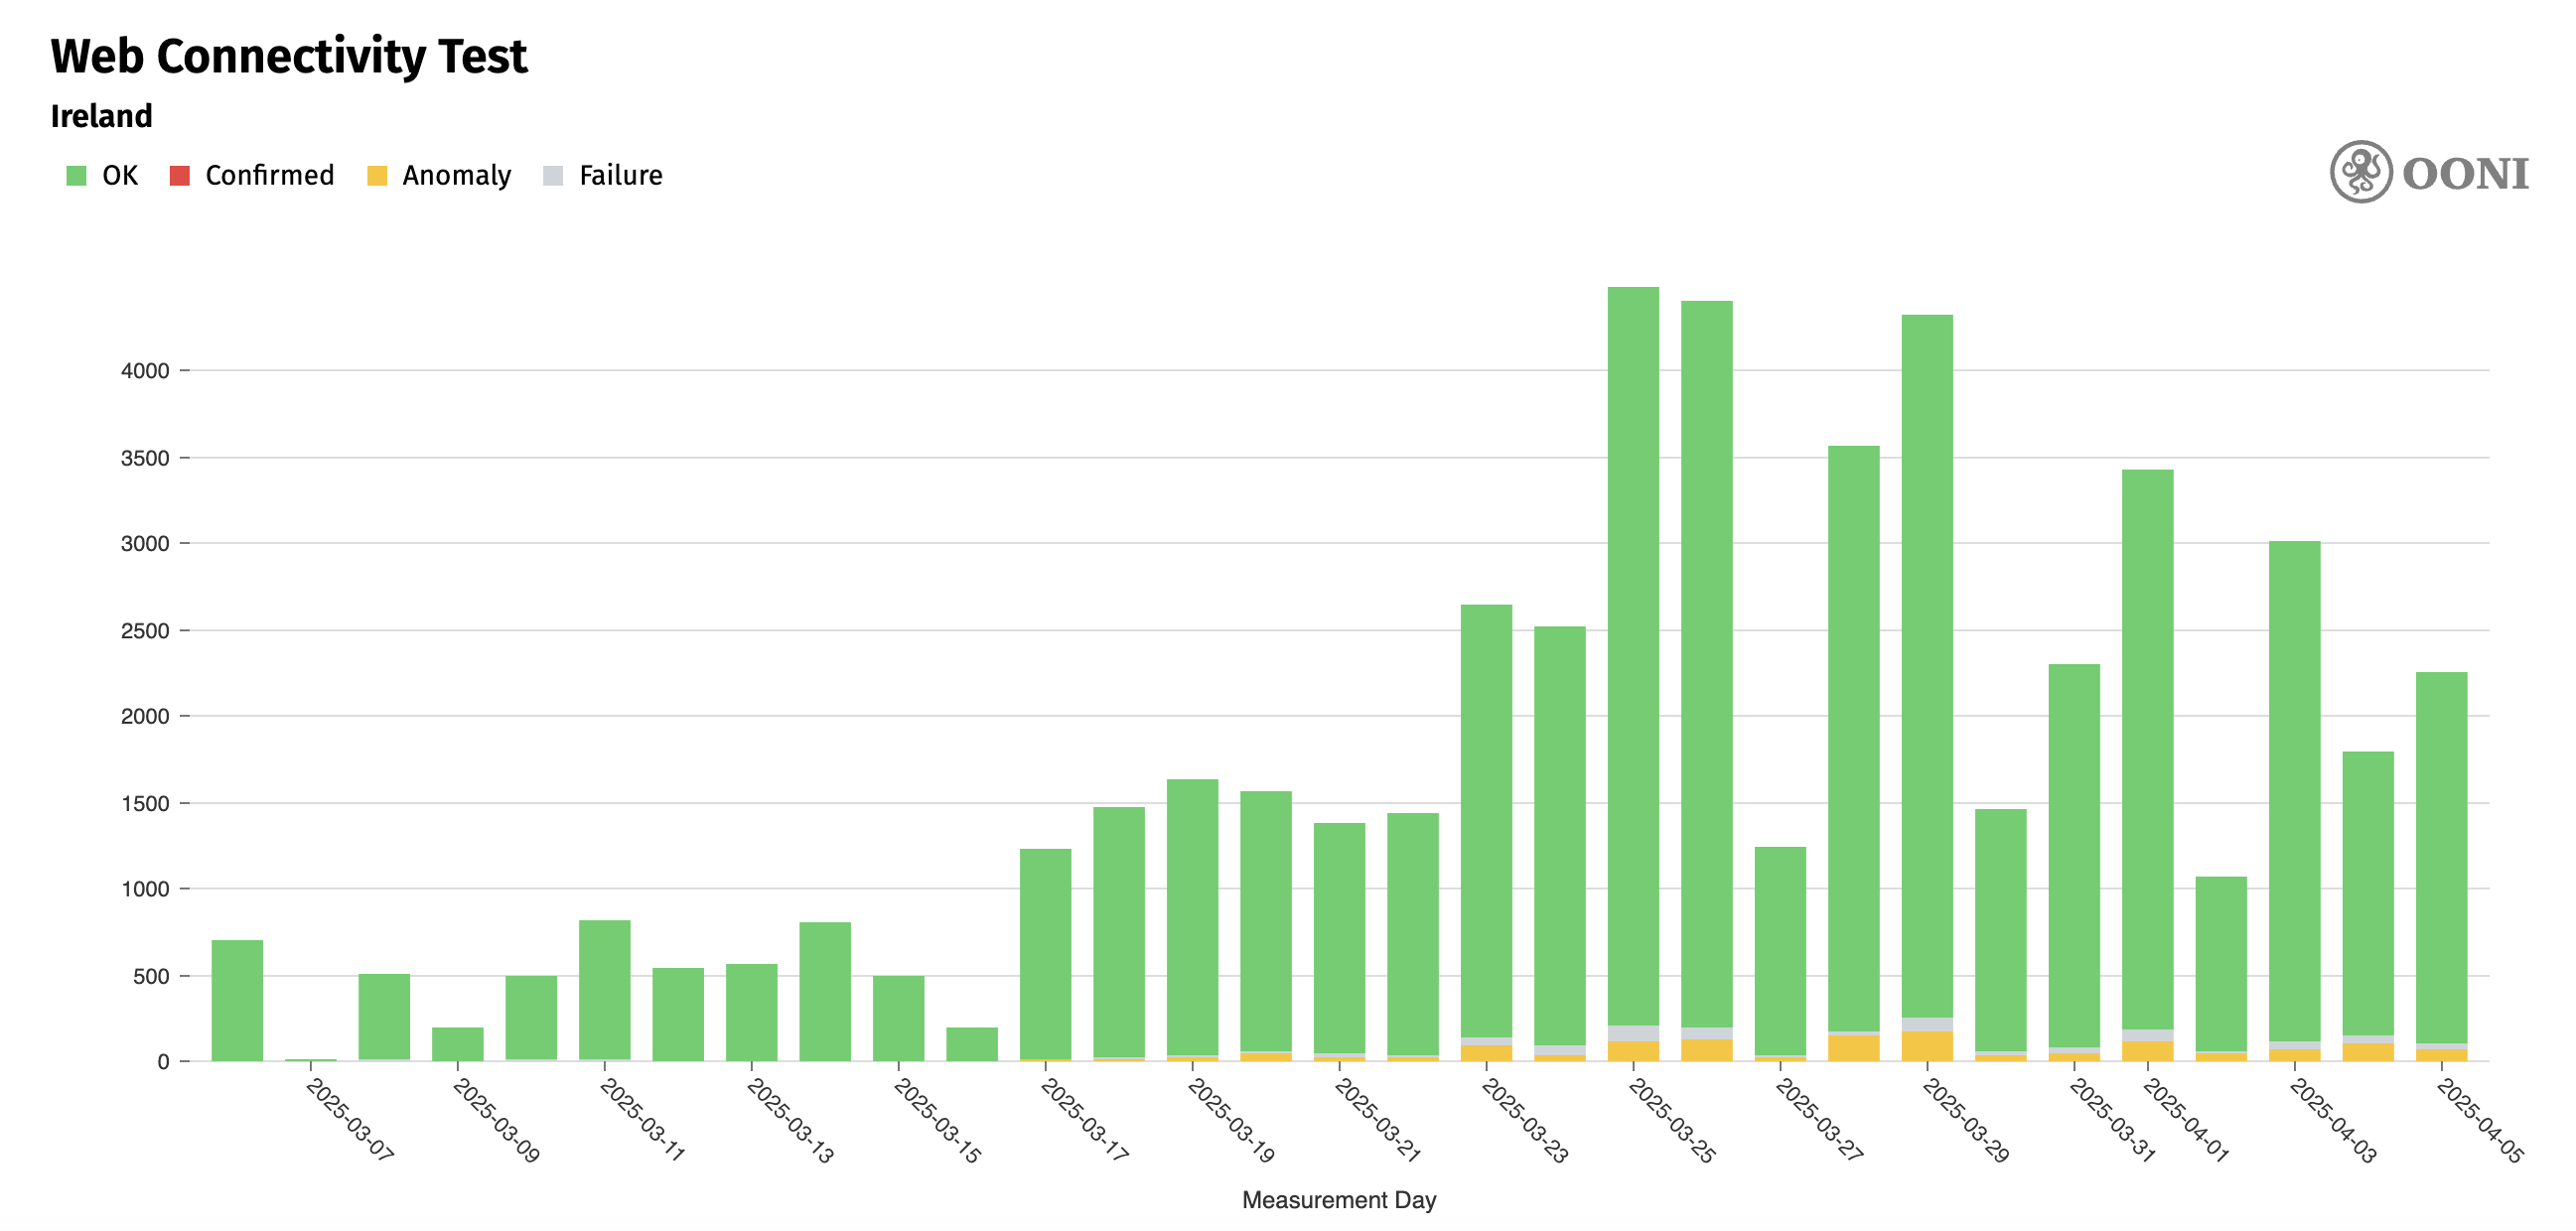
\includegraphics[width=\textwidth]{Griff/TCD SCSS CAPSTONE/Results/IrelandWebsiteTest.png}
    \caption{Ireland Web Connectivity Test: March 6, 2025 -- April 6, 2025}
    \label{fig:iraq-middlebox-HTTP-manipulation}
\end{figure}

\begin{figure}[H]
    \centering
    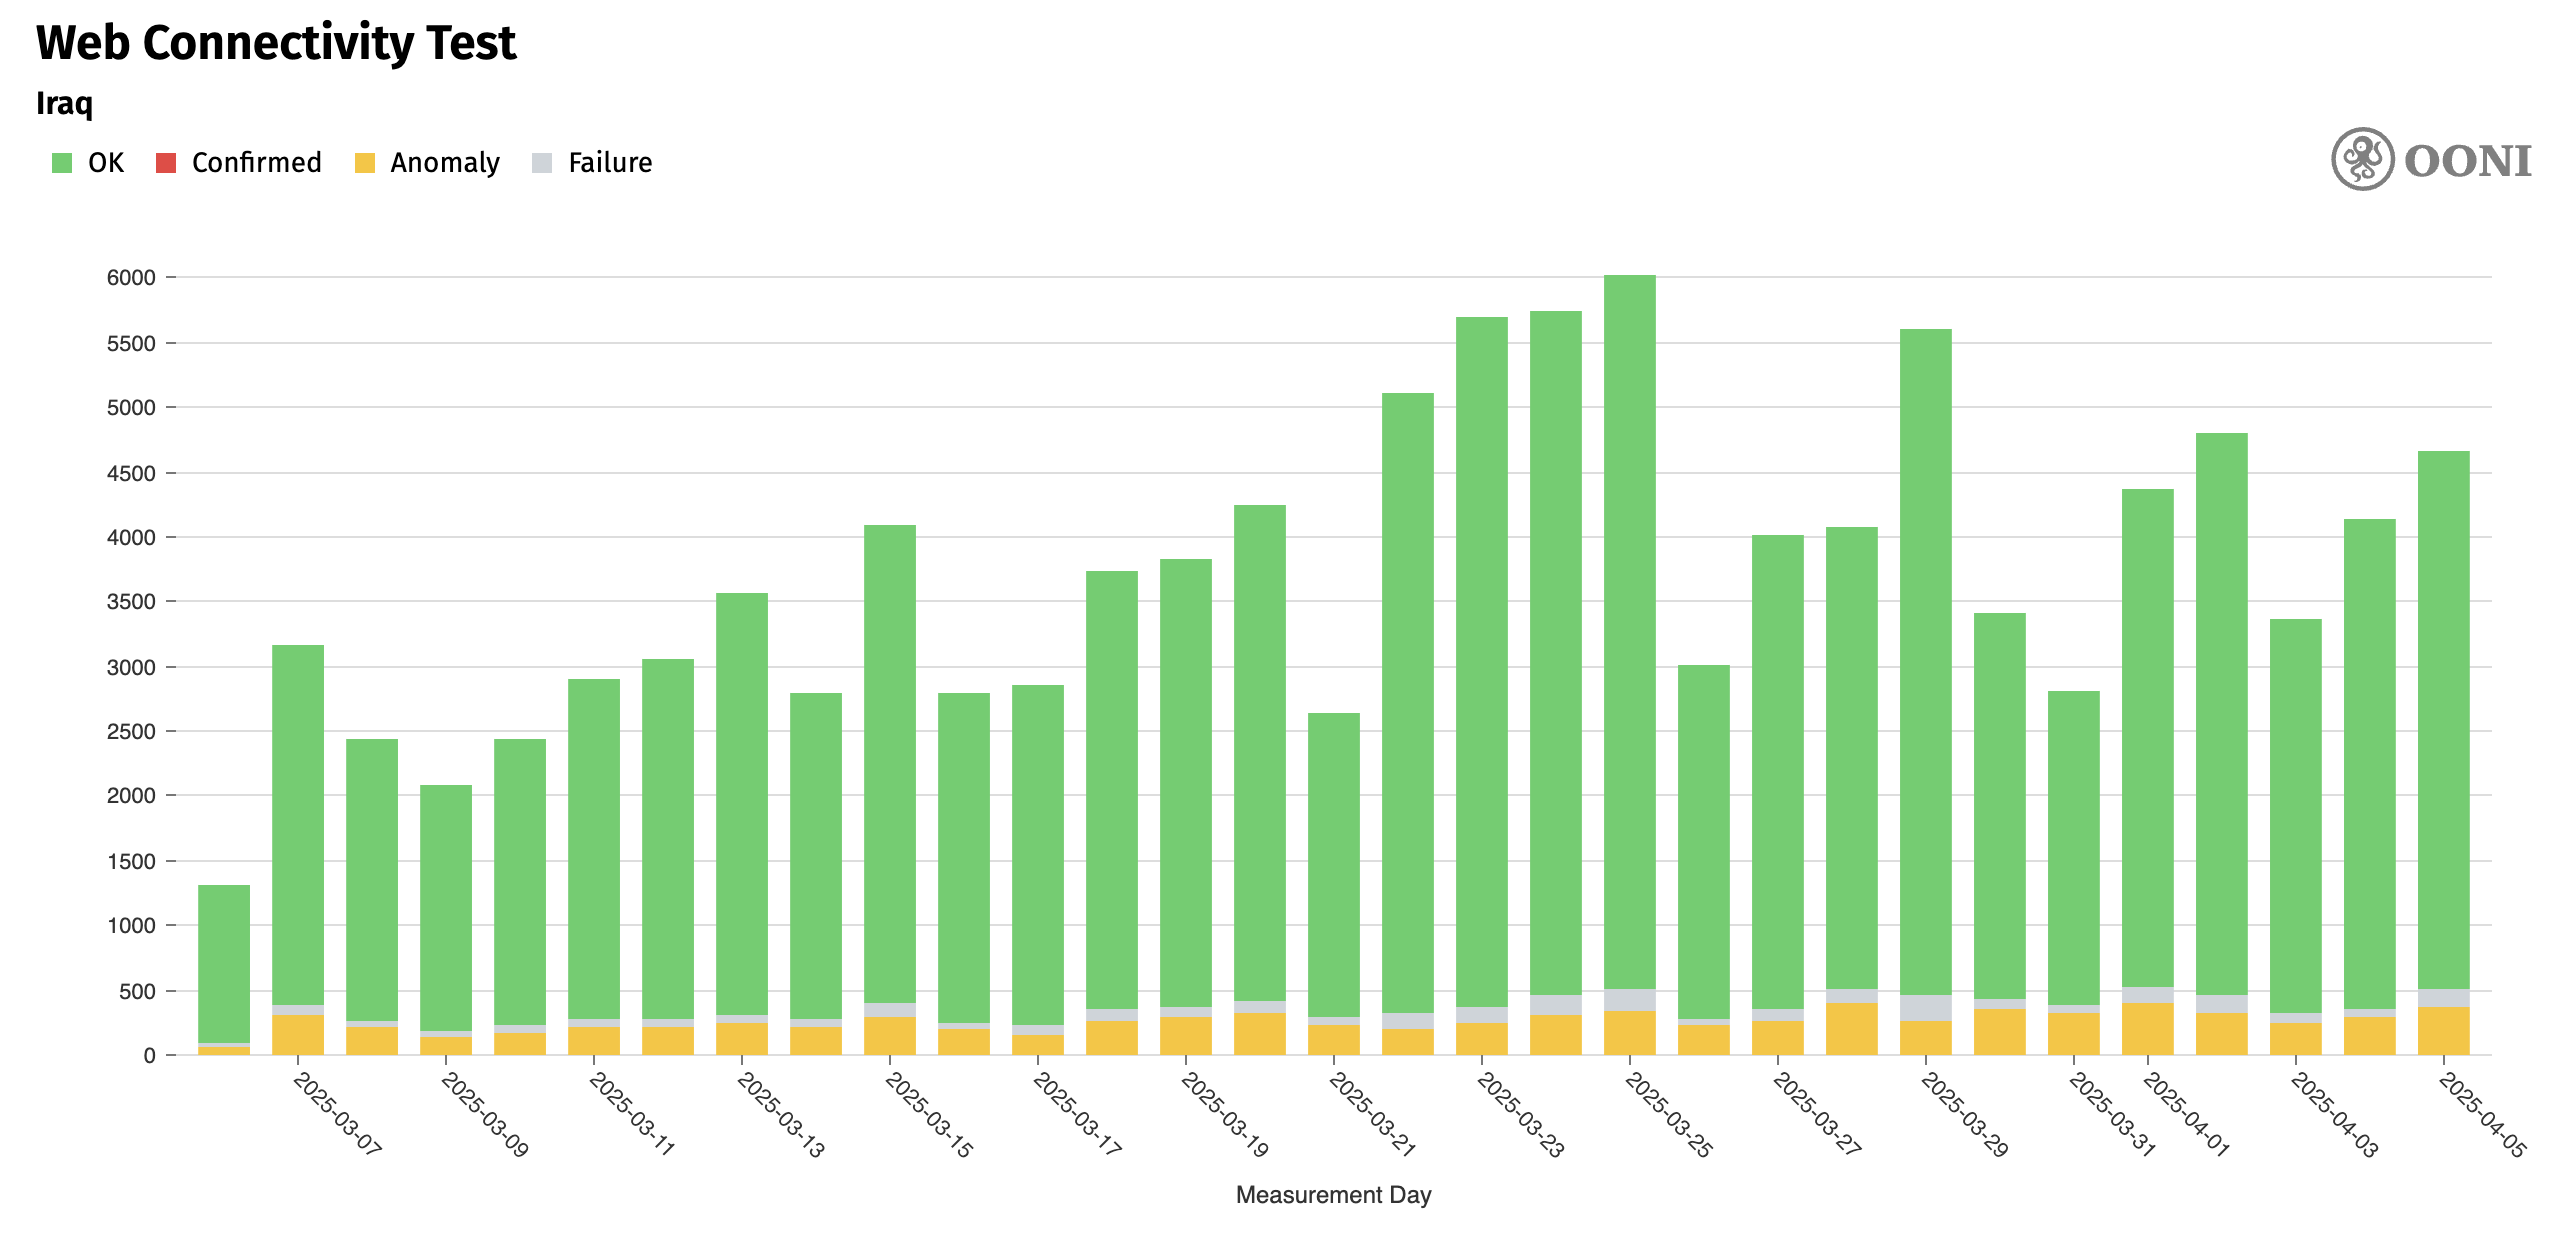
\includegraphics[width=\textwidth]{Griff/TCD SCSS CAPSTONE/Results/IraqWebsiteTest.png}
    \caption{Iraq Web Connectivity Test: March 6, 2025 -- April 6, 2025}
    \label{fig:iraq-middlebox-HTTP-manipulation}
\end{figure}

\subsection{Circumvention Test Results}

\subsubsection{Ireland}

Ireland likely does not block Tor on any ASNs, as it is largely accessible outside two anomalies.

\textbf{March 18, 2025} - Magnet Networks Limited (AS34245) - Tor Test (1 anomaly out of 78 measurements)
%https://explorer.ooni.org/m/20250318181530.182975_IE_tor_8b558463294b2881

\textbf{March 31, 2025} - Liberty Global B.V. (AS6830) - Tor Test (1 anomaly out of 191 measurements)
%https://explorer.ooni.org/m/20250331102020.562562_IE_tor_913ee551111fe0a9

Outside of these two anomalies, there is no evidence that Tor is being blocked in Ireland.

Psiphon, on the other hand, yielded different results. While Psiphon was largely able to be accessed on most ASNs, there were a few where access was likely blocked. 

\vspace{2em}

\begin{table}[H]
\centering
\caption{Networks in Ireland with Evidence of Psiphon Blocking}
\begin{tabular}{lccccc}
\toprule
\textbf{Network Name} & \textbf{ASN} & \shortstack{\textbf{Psiphon} \\ \textbf{Blocking Events}} & \shortstack{\textbf{Total} \\ \textbf{Measurements}} & \shortstack{\textbf{Block} \\ \textbf{Rate (\%)}} \\
\midrule
Microsoft Corporation           & AS8075  & 1  & 1   & 100\%  \\
HEAnet Ltd.                     & AS1213  & 33 & 35  & 94\%   \\
O2 Ireland Ltd.                 & AS13280 & 8  & 12  & 66\%   \\
Vodafone Ireland Ltd.           & AS15751 & 1  & 9   & 11\%   \\
Liberty Global B.V.             & AS6830  & 16 & 215 & 7.4\%  \\
\bottomrule
\textbf{Total} &  & \textbf{59} & \textbf{494} & \textbf{12.1\%} \\
\end{tabular}

\vspace{1em}

\caption*{\textit{Note:} "Psiphon Blocking Events" represent detected anomalies during testing of the Psiphon circumvention tool. "Block Rate" indicates the percentage of measurements that showed blocking behavior.}
\label{tab:psiphon_block_ireland}
\end{table}

\subsubsection{Iraq}

Like Ireland, Iraq does not block access to Tor, except for a few outliers.

\textbf{March 20, 2025} - Super Cell Network for Internet Services LTD (AS209193) - Tor Test (1 anomaly out of 92 measurements)
%https://explorer.ooni.org/m/20250320220102.873661_IQ_tor_3796e6aaa913670d

\textbf{March 30, 2025} - Hulum Almustakbal Company for Communication Engineering and Services Ltd (AS203214) - Tor Test (2 anomalies out of 160 measurements)
%https://explorer.ooni.org/m/20250330191838.341920_IQ_tor_f0e7ccd345c39d7f

\textbf{March 30, 2025} - Valin Company for General Trading and Communications LTD (AS205254) - Tor Test (1 anomaly out of 17 measurements)
%https://explorer.ooni.org/m/20250330111106.914884_IQ_tor_f45745fcedc21407

Outside of these anomalies, no significant evidence exists that Tor is being blocked in Iraq.

There is also little evidence of Psiphon being blocked in Iraq significantly. Aside from a few outliers, Psiphon only seemed to be blocked on one ASN. 

\vspace{2em}

\begin{table}[H]
\centering
\caption{Networks in Iraq with Evidence of Psiphon Blocking}
\begin{tabular}{lccccc}
\toprule
\textbf{Network Name} & \textbf{ASN} & \shortstack{\textbf{Psiphon} \\ \textbf{Blocking Events}} & \shortstack{\textbf{Total} \\ \textbf{Measurements}} & \shortstack{\textbf{Block} \\ \textbf{Rate (\%)}} \\
\midrule
HulumTele             & AS203214  & 127 & 165  & 77\%   \\
NB Telecom            & AS208324  & 1   & 3    & 33\%   \\
AsiaCell Telecom      & AS51684   & 4   & 23   & 17\%   \\
Valin Co LTD          & AS205254  & 1   & 30   & 3.3\%  \\
Earthlink Telecom     & AS199739  & 1   & 352  & 0.2\%  \\
\bottomrule
\textbf{Total}        &           & \textbf{134} & \textbf{1107} & \textbf{12.1\%} \\
\end{tabular}

\vspace{1em}

\caption*{\textit{Note:} "Psiphon Blocking Events" refer to instances where the Psiphon circumvention tool exhibited signs of interference. "Block Rate" is calculated as the percentage of blocked measurements over the total measured on each network.}
\label{tab:psiphon_block_iraq}
\end{table}

\subsection{Instant Messaging Test Results}

The results of the Instant Messaging tests were very similar in Ireland and Iraq. Both tests showed no signs of interference or blocking of Facebook Messenger, Telegram, Whatsapp, or Signal. However, looking outside the tested ASNs reveals a significant difference between the two countries. The tested data in Ireland is consistent with public OONI data and shows no blocking of instant messaging platforms. The Iraq data is also consistent with tests run on the same ASN, but in Iraq, other ASNs show signs of blocking.

\subsubsection{Ireland}

In the past 30-day period, there were only 2 anomalies found that shows any kind of instant messaging blocking:

\textbf{March 24, 2025} - Packethub S.A. (AS136787) - Facebook Messenger Test (1 anomaly out of 3 measurements)
%https://explorer.ooni.org/m/20250324111124.418686_IE_facebookmessenger_fbdc8895400acaba

\textbf{March 24, 2025} - HEAnetCLG (AS1213) - Signal Test (1 anomaly out of 37 measurements)
%https://explorer.ooni.org/m/20250324164458.153631_IE_signal_667f7ad13e55043a

Outside of these anomalies, there was no evidence of instant messaging blocking.

\subsubsection{Iraq}

Iraq had significant evidence of instant messaging platforms being blocked in certain ASNs. The table below shows each ASN and the percentage of tests where an anomaly was found.

\vspace{2em}

\begin{table}[H]
\centering
\caption{Networks in Iraq with Evidence of Instant Messaging Platform Blocking}
\begin{tabular}{lcccccc}
\toprule
\textbf{Network Name} & \textbf{ASN} & \shortstack{\textbf{Facebook} \\ \textbf{Block Rate}} & \shortstack{\textbf{Telegram} \\ \textbf{Block Rate}} & \shortstack{\textbf{WhatsApp} \\ \textbf{Block Rate}} & \shortstack{\textbf{Signal} \\ \textbf{Block Rate}} \\
\midrule
CIT Co LTD            & AS212330  & 100\% & 0\%   & 0\%   & 0\%   \\
KNET                  & AS206206  & 60\%  & 0\%   & 0\%   & 0\%   \\
Cloudflare, Inc.      & AS13335   & 47\%  & 0\%   & 0\%   & 0\%   \\
Earthlink Telecom     & AS50710   & 33\%  & 0\%   & 0\%   & 0\%   \\
HulumTele             & AS203214  & 27\%  & 7.8\% & 25\%  & 44\%  \\
Valin Co LTD          & AS205254  & 26\%  & 3.8\% & 7.6\% & 7.6\% \\
Al-Nazeera Co.        & AS51020   & 0\%   & 0\%   & 0\%   & 32\%  \\
Noor Al-Bedaya Co.    & AS202651  & 0\%   & 0\%   & 0\%   & 23\%  \\
TLLG Co.              & AS210022  & 0\%   & 0\%   & 0\%   & 82\%  \\
Al Atheer Co. LTD     & AS59588   & 0\%   & 0\%   & 1.9\% & 1.9\% \\
Earthlink Telecom     & AS199739  & 1\%   & 0.5\% & 0.2\% & 0.8\% \\
Super Cell            & AS209193  & 0\%   & 0\%   & 0.7\% & 0\%   \\
\bottomrule
\textbf{Total Block Rate} & & \textbf{6.2\%} & \textbf{1.4\%} & \textbf{4.1\%} & \textbf{6.2\%} \\
\end{tabular}

\vspace{1em}

\caption*{\textit{Note:} Each percentage reflects the proportion of measurements on the respective network where blocking behavior was detected for a specific instant messaging platform. The platforms analyzed include Facebook Messenger, Telegram, WhatsApp, and Signal.}
\label{tab:im_block_iraq}
\end{table}

\subsection{Middlebox Test Results}

The results of the Middlebox Test were the same for both countries. Both the HTTP Header Field Manipulation and HTTP Invalid Request Line tests detected no Middleboxes in either country. However, while there was no evidence of Middleboxes being found using the providers tested, it is possible that other providers in both countries have Middleboxes present in the network.

Using publicly available OONI data for Ireland and Iraq, it was found that Middleboxes were detected in both countries over the past 30 days (March 6, 2025 - April 6, 2025). 

\subsubsection{Ireland}

There is very little evidence of Middleboxes in Ireland. Over the past 30-day period, only two anomalies have been present. Both of these anomalies are from the HTTP Invalid Request Line test. 

\textbf{March 25, 2025} - Meteor Mobile Communications Ireland (AS15751) (1 anomaly out of 9 measurements)
%https://explorer.ooni.org/m/20250325122211.663367_IE_httpinvalidrequestline_c713442d98eebb5c

\textbf{April 1, 2025} - Vodafone Ireland Limited (AS15502) (1 anomaly out of 79 measurements)
%https://explorer.ooni.org/m/20250401215651.365763_IE_httpinvalidrequestline_51f20fe7e9d31698

These results are likely outliers, as there were very few Middlebox tests for Meteor Mobile Communications Ireland during this time span and no other anomalies for Vodafone Ireland Limited.

\subsubsection{Iraq}

There is considerably more evidence of Middleboxes in Iraq. Over the past 30 days, there were 125 anomalies in the HTTP Invalid Request line Test and 19 anomalies in the HTTP Header Field Manipulation Test.

The table below lists the ASNs suspected to have Middleboxes present using the HTTP Invalid Request Line test. It then shows the number of anomalies, the total measurement count, and the percentage of the total count that was anomalies.

\vspace{2em}

\begin{table}[H]
\centering
\caption{Networks in Iraq with Evidence of Middleboxes (HTTP Invalid Request Line Test)}
\begin{tabular}{lccccc}
\toprule
\textbf{Network Name} & \textbf{ASN} & \shortstack{\textbf{Detected} \\ \textbf{Events}} & \shortstack{\textbf{Total} \\ \textbf{Measurements}} & \shortstack{\textbf{Block} \\ \textbf{Rate (\%)}} \\
\midrule
EarthLink Ltd.        & AS50710   & 1  & 1   & 100\%    \\
Al-Jazeera Co.        & AS198589  & 68 & 70  & 97\%     \\
Cloudflare, Inc.      & AS13335   & 8  & 10  & 80\%     \\
IQ-Online             & AS48492   & 2  & 4   & 50\%     \\
Al Atheer Co. LTD     & AS59588   & 13 & 53  & 24.5\%   \\
HulumTele             & AS203214  & 32 & 158 & 20.25\%  \\
\bottomrule
\textbf{Total} & & \textbf{125} & \textbf{1071} & \textbf{11.6\%} \\
\end{tabular}

\vspace{1em}

\caption*{\textit{Note:} This table presents results from the HTTP Invalid Request Line Test. "Detected Events" refer to anomalies suggesting the presence of network middleboxes. "Block Rate" is the percentage of such events relative to the total measurements per ASN.}
\label{tab:middlebox_http_invalid}
\end{table}

%\begin{figure}[H]
%    \centering
%    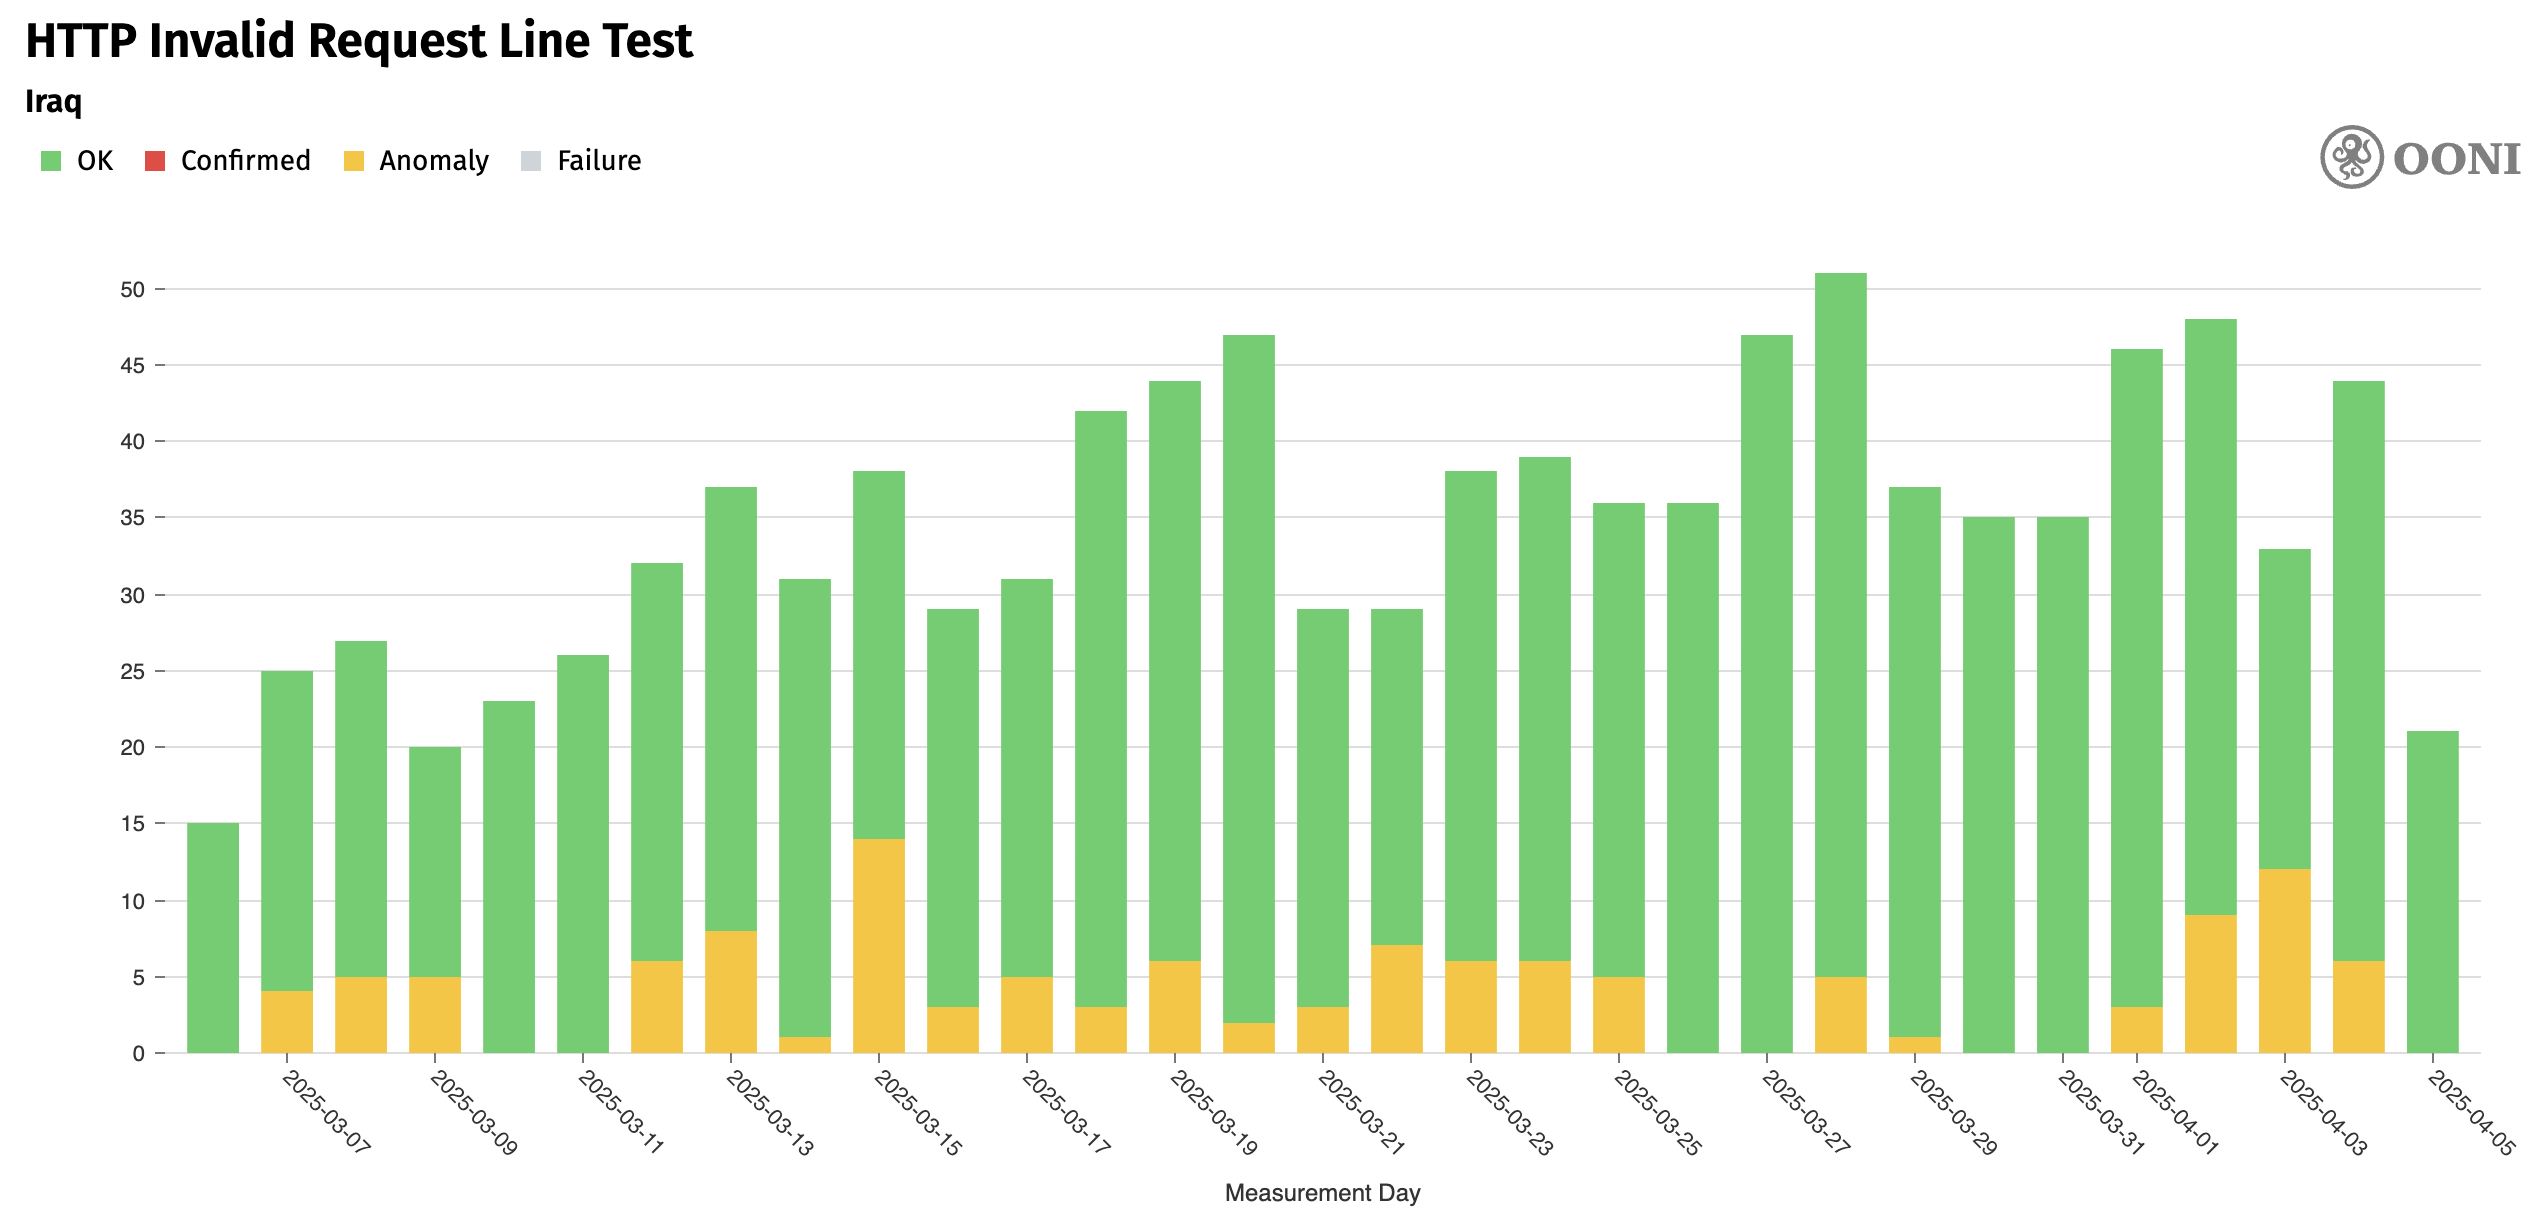
\includegraphics[width=\textwidth]{Griff/TCD SCSS CAPSTONE/Results/IraqMiddleboxHTTPInvalidTest.png}
 %   \caption{Iraq Middlebox HTTP Invalid Request Line Test: March 6, 2025 -- April 6, 2025}
%    \label{fig:iraq-middlebox-invalid-request}
%\end{figure}

The table below lists the ASNs suspected to have Middleboxes present using the HTTP Header Field Manipulation test. It then shows the number of anomalies, the total measurement count, and what percentage of the total count were anomalies. Note that any ASN that had less than 0.5\% anomalies was ignored.

\vspace{2em}

\begin{table}[H]
\centering
\caption{Networks in Iraq with Evidence of Middleboxes (HTTP Header Field Manipulation Test)}
\begin{tabular}{lccccc}
\toprule
\textbf{Network Name} & \textbf{ASN} & \shortstack{\textbf{Detected} \\ \textbf{Events}} & \shortstack{\textbf{Total} \\ \textbf{Measurements}} & \shortstack{\textbf{Block} \\ \textbf{Rate (\%)}} \\
\midrule
EarthLink Ltd.        & AS50710  & 1 & 1  & 100\%  \\
Cloudflare, Inc.      & AS13335  & 8 & 10 & 80\%   \\
IQ-Online             & AS48492  & 2 & 4  & 50\%   \\
\bottomrule
\textbf{Total} & & \textbf{11} & \textbf{15} & \textbf{1.7\% of full dataset (1074)} \\
\end{tabular}

\vspace{1em}

\begin{minipage}{0.95\linewidth}
\caption*{\textit{Note:} This test detects potential middleboxes by observing anomalies in how HTTP header fields are processed. "Detected Events" are instances of irregular responses, possibly caused by network interference. "Block Rate" indicates the ratio of these events to total measurements per ASN.}
\end{minipage}
\label{tab:middlebox_http_header}
\end{table}

%\begin{figure}[H]
 %   \centering
%    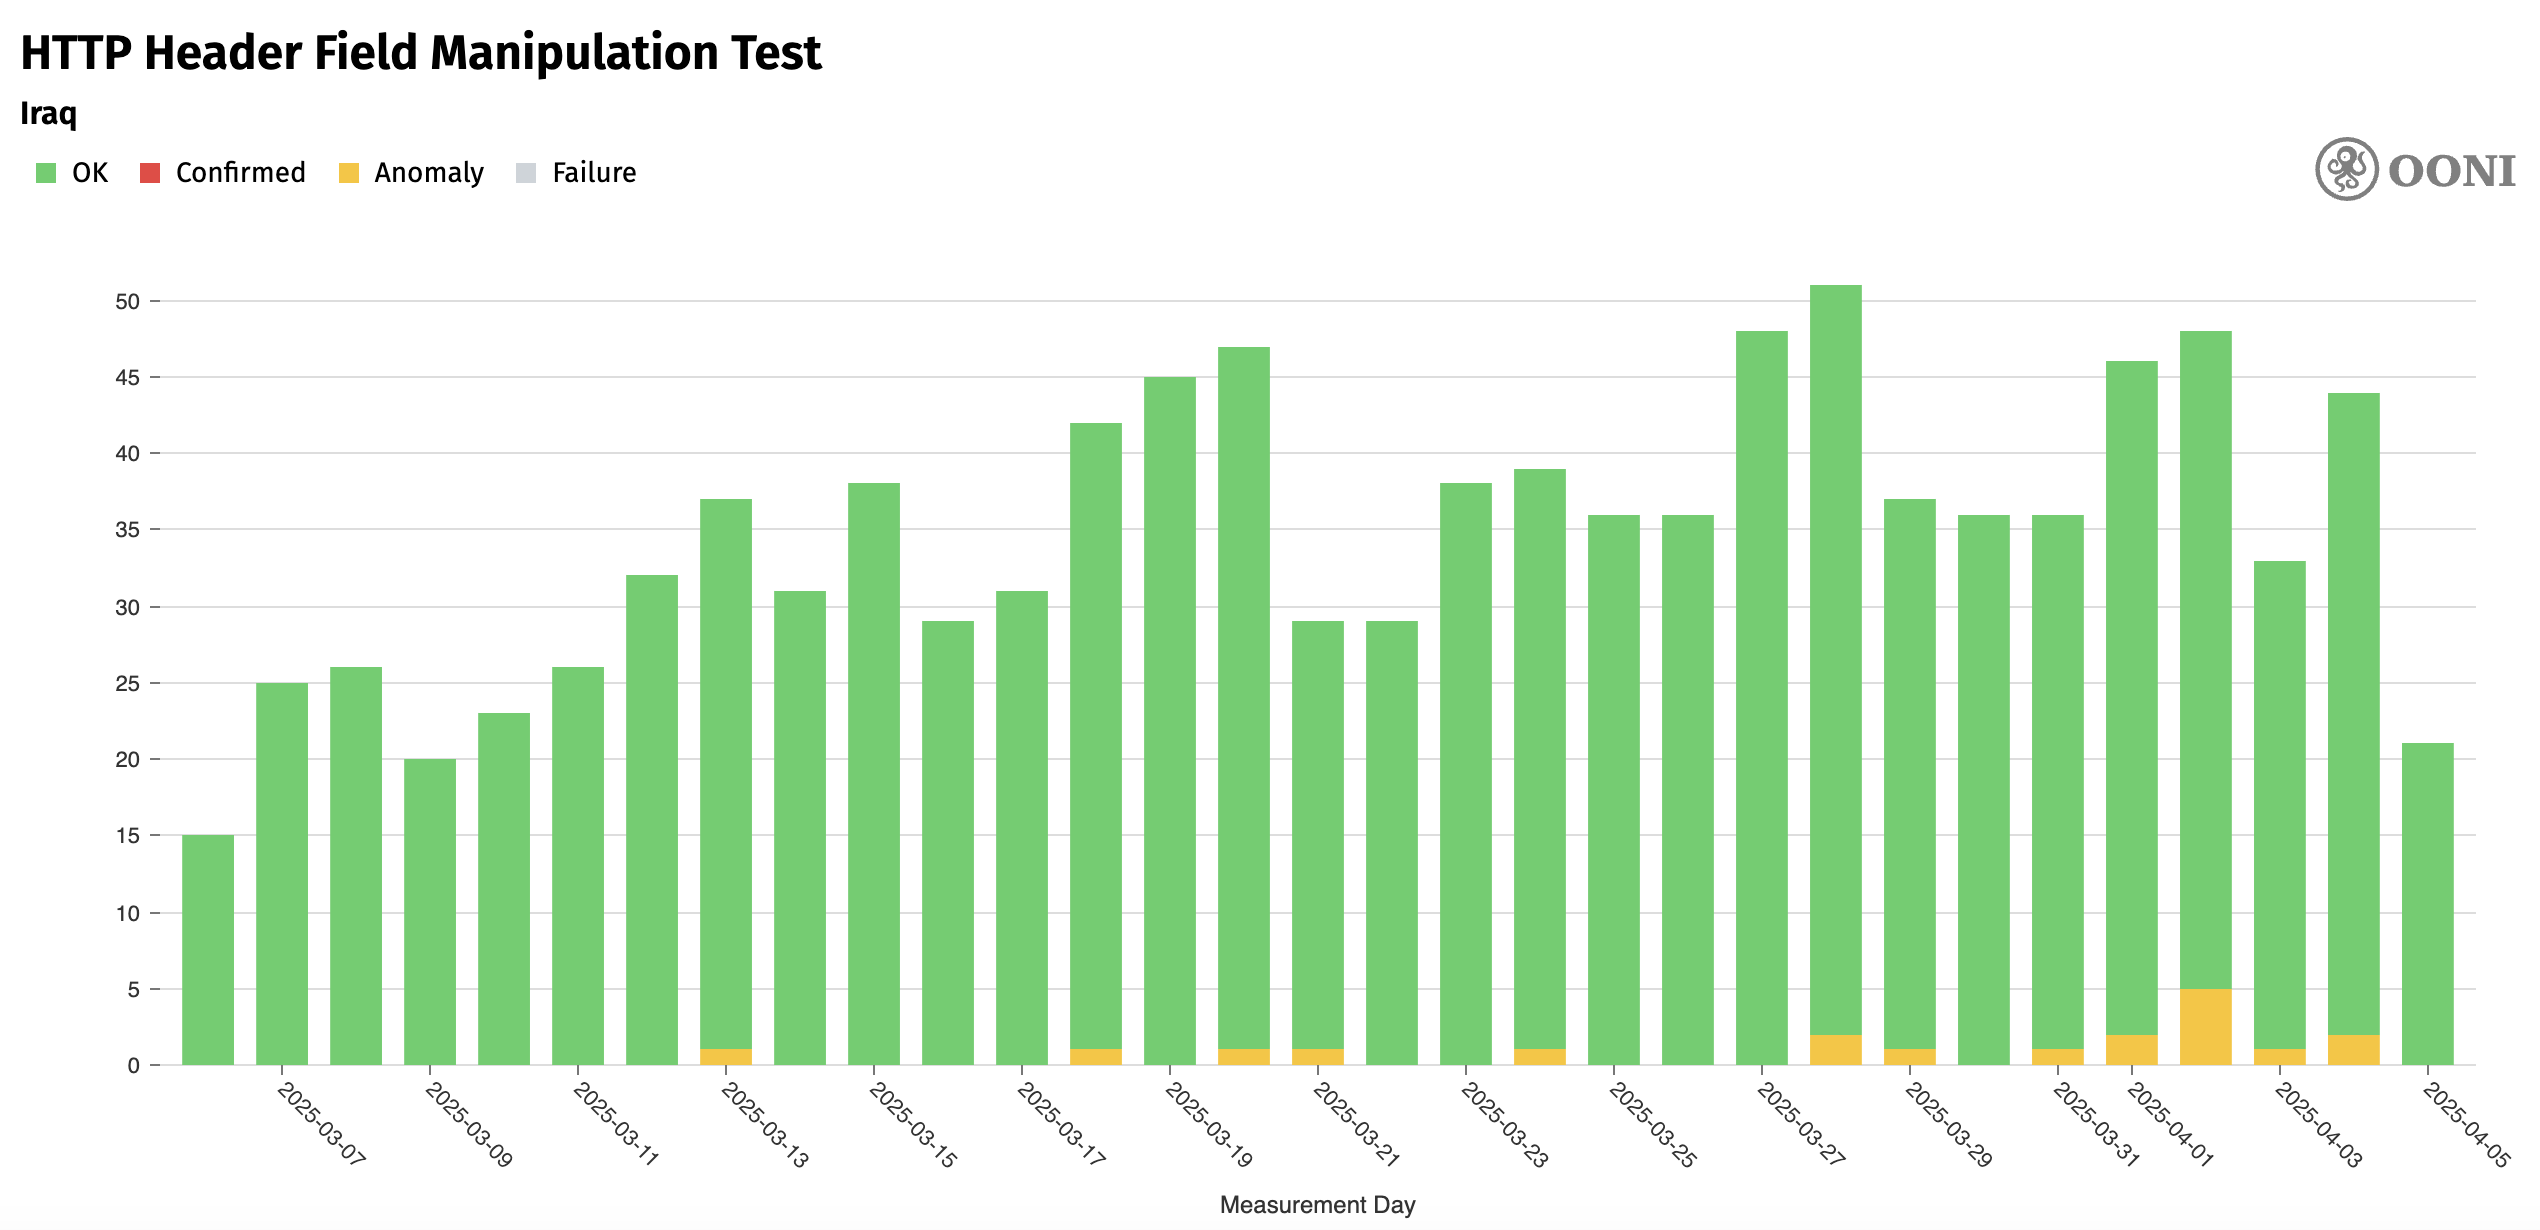
\includegraphics[width=\textwidth]{Griff/TCD SCSS CAPSTONE/Results/IraqMiddleboxHTTPManipulation.png}
%    \caption{Iraq Middlebox HTTP Header Field Manipulation Test: March 6, 2025 -- April 6, 2025}
%    \label{fig:iraq-middlebox-HTTP-manipulation}
%\end{figure}

\textit{Note: All CSV files gathered from the public OONI database can be found on the public GitHub for this work; see Appendix A1.2.}


\section{Comparative Analysis: Ireland v. Iraq}

The combined results of OONI probe testing and public OONI data reveal differences in censorship between Ireland and Iraq. While both countries implement content restrictions and other blocks, there are significant differences in the scale and motivations behind these blocks.

\subsubsection{Website Accessability}
\label{sec:Website-Accessability-Analysis}

The manually run web connectivity test yielded unexpected results. The proportion of blocked websites in both countries was similar, with Ireland having a slight edge over Iraq. This was unexpected, but because these tests were run manually on only one or two networks in each country, these results may only give a partial view of the country's Internet censorship. The results become more expected when looking at the publicly available OONI data. In the 30 days, Iraq blocked significantly more websites than Ireland and at a higher rate. Of the 3703 websites tested in Iraq, 262 had anomalies (7\% blocking rate), while of the 1695 websites tested in Ireland, only 43 had anomalies (2.5\% blocking rate). Looking at the figures, it is clear that Iraq blocks more content and on a more consistent basis than Ireland.

The blocking rates of websites by category reveal more expected results. Ireland blocked significantly more Piracy / Streaming / File Sharing websites outside of uncategorized websites than Iraq, which aligns with Ireland's court-mandated approach to censorship. Conversely, Iraq blocked a wider range of content by category, with a significant blocking rate of religious websites (75\%).

TCP/IP blocking was the top blocking method in both countries, indicating simple censorship mechanisms. Ireland, however, had a significantly higher rate of DNS blocking, which is likely due to its approach to targeted website blocking and EU compliance.

\subsubsection{Circumvention Tools}

The accessibility of Tor and Psiphon was essentially the same in Ireland and Iraq, with a few exceptions. Tor was widely accessible in both countries, indicating that Ireland and Iraq have no significant mechanisms to block this tool. If they do, there is no evidence that it is effective. There is evidence that Psiphon is blocked on specific ASNs in both countries, with public OONI data backing this up. In Ireland, Psiphon is blocked on HEAnet CLG (AS1213), as indicated by manually tested and public data. Over the same 30-day period, Ireland and Iraq blocked Psiphon 12.1\% of the time. As a result, there is little evidence of systemic efforts to block access to Psiphon, similar to Tor.

\subsubsection{Instant Messaging Platforms}

In Ireland, there is no evidence that instant messaging services are blocked meaningfully. This is in line with Ireland's stance on censorship and was expected. In Iraq, however, there is evidence that instant messaging services are blocked in some areas, but according to public OONI data, they are widely accessible. Some ASNs had implemented blocks on all four services tested to some capacity, indicating regional blocking in response to specific events. This is aligned with Iraq's more reactionary censoring practice.

\subsubsection{Presence of Middleboxes}

The use of Middleboxes in Ireland was almost non-existent, as there were only two anomalies over the 30-day period. These were likely false positives. This data indicates that Ireland does not implement TLS or SNI-based filtering systematically or widely. By contrast, Iraq showed significant evidence of Middleboxes being present. AS198589 showed significant signs of Middleboxes being present, and other ASNs have significant anomalies. This indicates that Iraq may implement TLS or SNI-based filtering in some areas of the country, which makes sense as we know that much of Iraq's current censorship efforts are decentralized. 

\subsection{Summary of Comparative Observations}

\begin{table}[H]
\centering
\caption{Comparative Summary of Internet Censorship: Ireland vs. Iraq}
\begin{tabular}{lcc}
\toprule
\textbf{Metric} & \textbf{Ireland} & \textbf{Iraq} \\
\midrule
Block Rate (OONI) & 2.5\% & 7\% \\
Blocking Methods & TCP/IP, DNS & TCP/IP, DNS, SNI \\
Tool Blocking & Rare, selective & Targeted, ASN-specific \\
Messaging Blocking & Negligible & Present on some ASNs \\
Middleboxes Detected & Minimal & Present on some ASNs \\
Motivations & Legal, EU compliance & Political, cultural control \\
\bottomrule
\end{tabular}
\label{tab:comparison_summary}
\end{table}

These findings support the initial research, showing that Ireland and Iraq have different censorship approaches. Ireland maintains a limited, legal-centric censorship model that is transparent and aligned with most other Western nations. Iraq's approach, while less centralized, is more reactive and inconsistent, often tied to internal events. 

\subsection{Future Work}

During this work, it became clear that exporting detailed public OONI data for web connectivity tests would be difficult. This public data would have provided more detailed insights into the differences between Ireland and Iraq. Future research could gather this data using the OONI public API to build upon this work. Using this API would allow for the automated collection of web connectivity data in Ireland and Iraq, giving the writer a broader foundation for comparison. This data would include blocking types, website categories, and ASN information.

Incorporating this public OONI data would facilitate a more holistic analysis of each country, as manual testing is only limited to one geographical location. This work shows that OONI tests yield different results in different regions of both countries, so relying solely on manually collected web connectivity data only gives a partial view of a country's current internet censorship. 
\chapter{Security and Privacy}

This section addresses security and privacy concerns involved with operating the OONI probe in relation to this work while considering both the technical aspects and the broader legal or regulatory aspects. The comparison of censorship between Ireland and Iraq is significant. While using the OONI probe within both countries comes with its own risk, the use of the probe in Iraq carries much more concern when it comes to security and privacy. The environment in Iraq is significantly more dangerous with ongoing government surveillance, frequent shutting down of social media sites, and the risk of authorities considering unauthorized data-gathering activities as suspicious. All these factors indicate the need to carefully plan where, how, and why measurements are taken, as well as how resulting data will be stored.

\section{OONI}

Although OONI strives to minimize the collection of personal data, its measurements are published openly, which may inadvertently disclose approximate locations and times when tests occurred \cite{ooniOONIPrivacyAndSecurity}. If the individual running OONI is tied to a VM in Iraq with an IP address, local authorities or ISPs might link test activity back to the source. This risk is particularly heightened if the probe is frequently connecting to or testing politically sensitive, banned, or controversial websites. In a high-censorship environment, repeated network tests can attract attention and might be interpreted as an intentional challenge to government policies.

\section{Iraq Virtual Machine}

When deploying a VM in Iraq, the potential security and privacy risk increases due to the possibility that authorities or other outside sources might attempt to compromise the server. The government of Iraq might be motivated to confiscate or check the contents of the VM in order to identify individuals who are actively monitoring sensitive network interference. It is also possible that the hosting provider itself can be forced to give logs, user connections, or site testing targets, which removes all privacy the user has. To avoid this, one should ensure that no personal data is used on this VM, and tools for circumvention are used to encrypt the origin of the user accessing the VM.

Even beyond direct government intervention, there is the risk of third-party hacks or malware injection. A public and well known measurement platform like OONI will attract hackers looking to disrupt users of this tool or introduce malware that will capture all incoming and outgoing traffic. In Iraq, the network infrastructure might already contain middleboxes or deep packet inspection systems that are actively filtering or manipulating data. These devices sometimes disrupt the traffic generated by the OONI probe measurements, leading to manipulated data to be collected.

\section{Legal Risks}




\chapter{Conclusions}

This work set out to research and compare internet censorship practices in Ireland and Iraq. These two nations have significantly different governments and cultures. By using both direct network testing using the OONI Probe and published OONI data, this work has identified the distinct methods and motivations behind censorship in each country. 

Ireland as a member of the European Union implements a limited and legally rooted censorship model. Ireland mainly blocks illegal and pirated content, and these blocks are implemented through the country's legal system or through EU compliance. The OONI data shows that there is little evidence of widespread censorship of non-illegal content, no use of advanced censorship methods like TLS / SNI-based filtering, and no efforts to block circumvention tools.

Iraq implements a more decentralized and reactionary censorship model, where a wider range of content is blocked when compared to Ireland. The Iraqi government is known to shut off internet access in parts of the country during times of unrest or national exams. The OONI data shows that there is evidence TLS/ SNI-based filters in specific parts of the country, but there is no evidence to support that there is widespread implementation of these advanced mechanisms. Additionally there is some evidence of some circumvention tools, such as Psiphon, being blocked in some areas, but there is nothing to support widespread efforts to block these tools. These findings point to regional and situational censorship, driven by political or cultural events rather than being rooted in a legal basis.

This comparative analysis contributes to the growing importance of digital rights and government accountability by using empirical data and structured analysis. The importance of projects like OONI allows for people to learn about the presence and nature of internet censorship in their own countries, and gives researchers the ability to identify global trends and document network interference. As the internet continues to grow in importance to civil discourse, education, and access to information, vigilance against censorship becomes foundational.

\bibliographystyle{unsrtnat}
\bibliography{bibs/sample}

\appendix
\renewcommand{\thechapter}{A\arabic{chapter}}
\chapter{Appendix}
\begin{figure} [H]
    \centering
    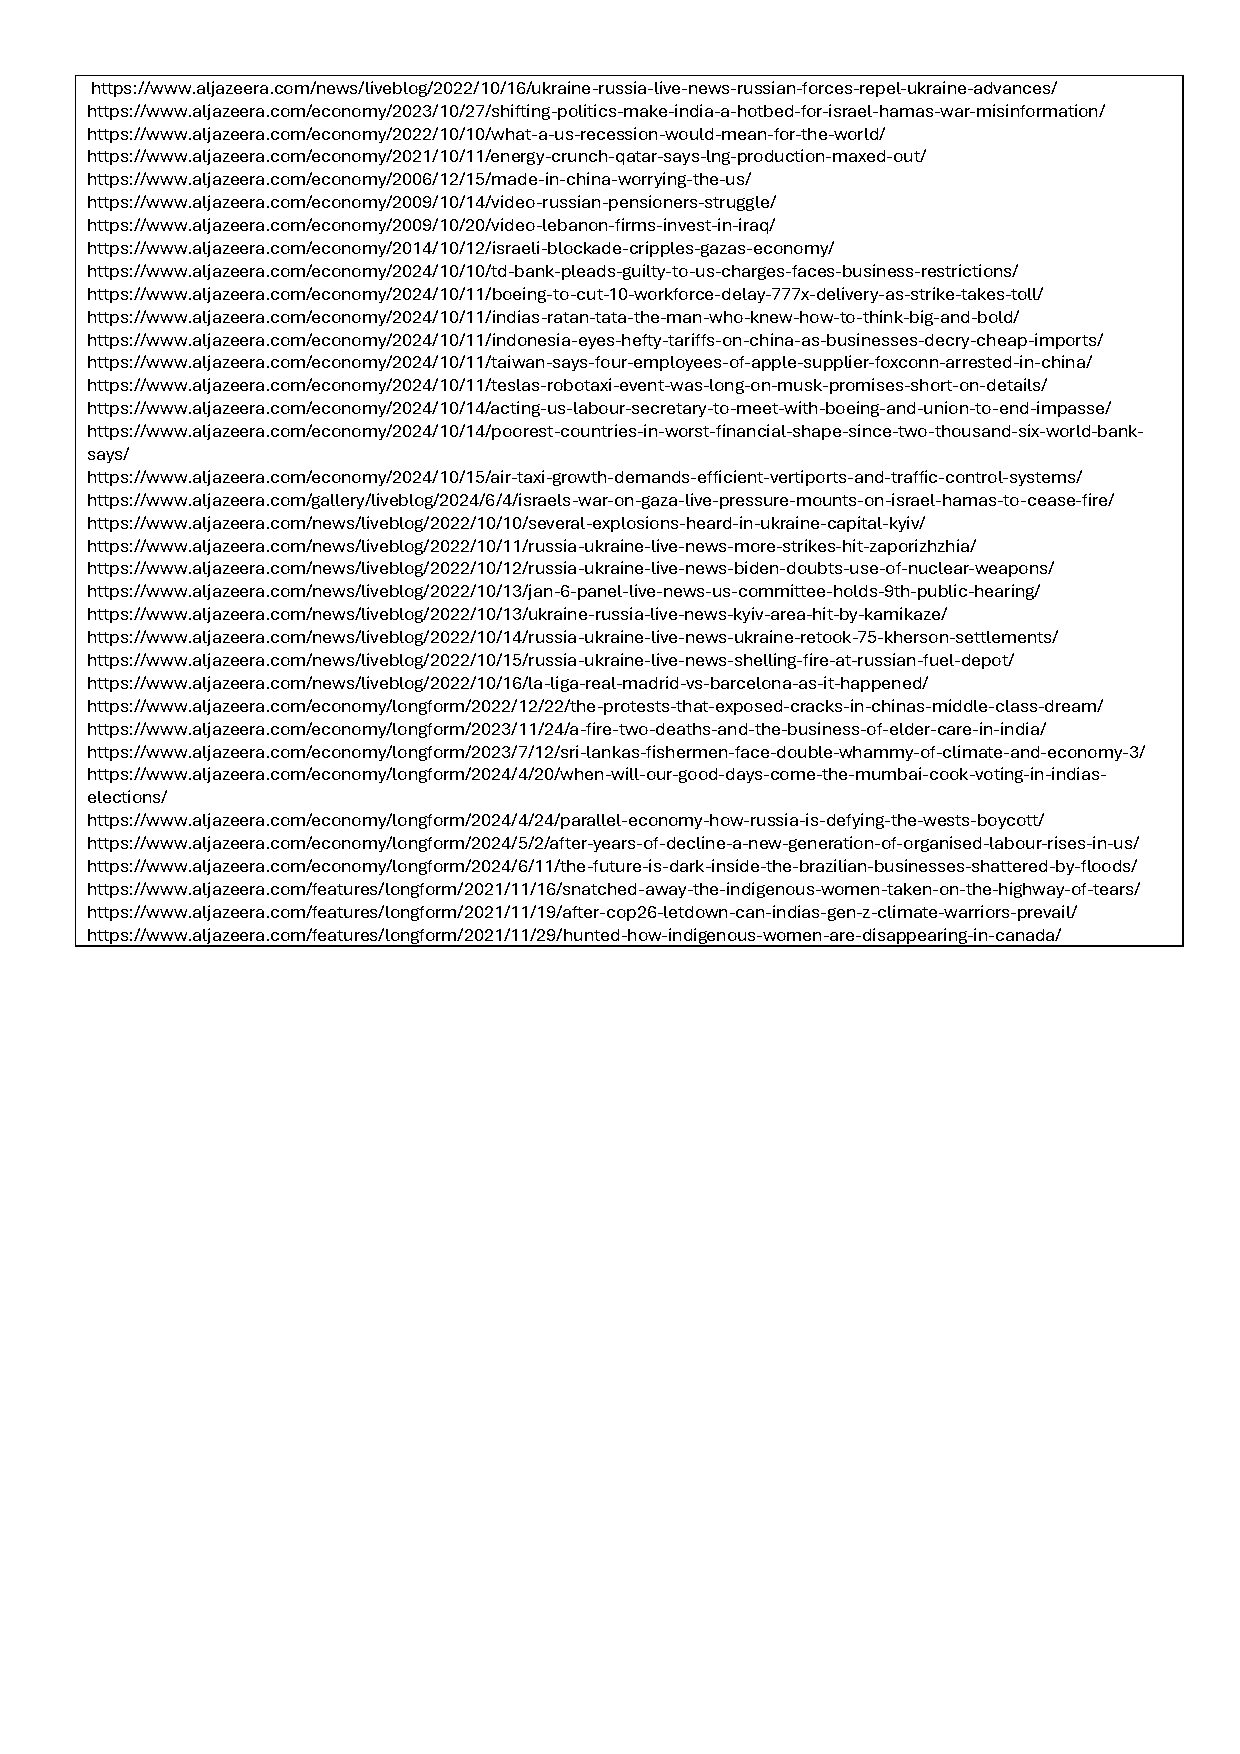
\includegraphics[width=0.8\linewidth]{sample-aljazeera.pdf}
    \caption{sample-aljazeeraurls.txt contains URLs scraped from aljazeera.com}
    \label{fig:enter-label}
\end{figure}

\begin{figure} [H]
    \centering
    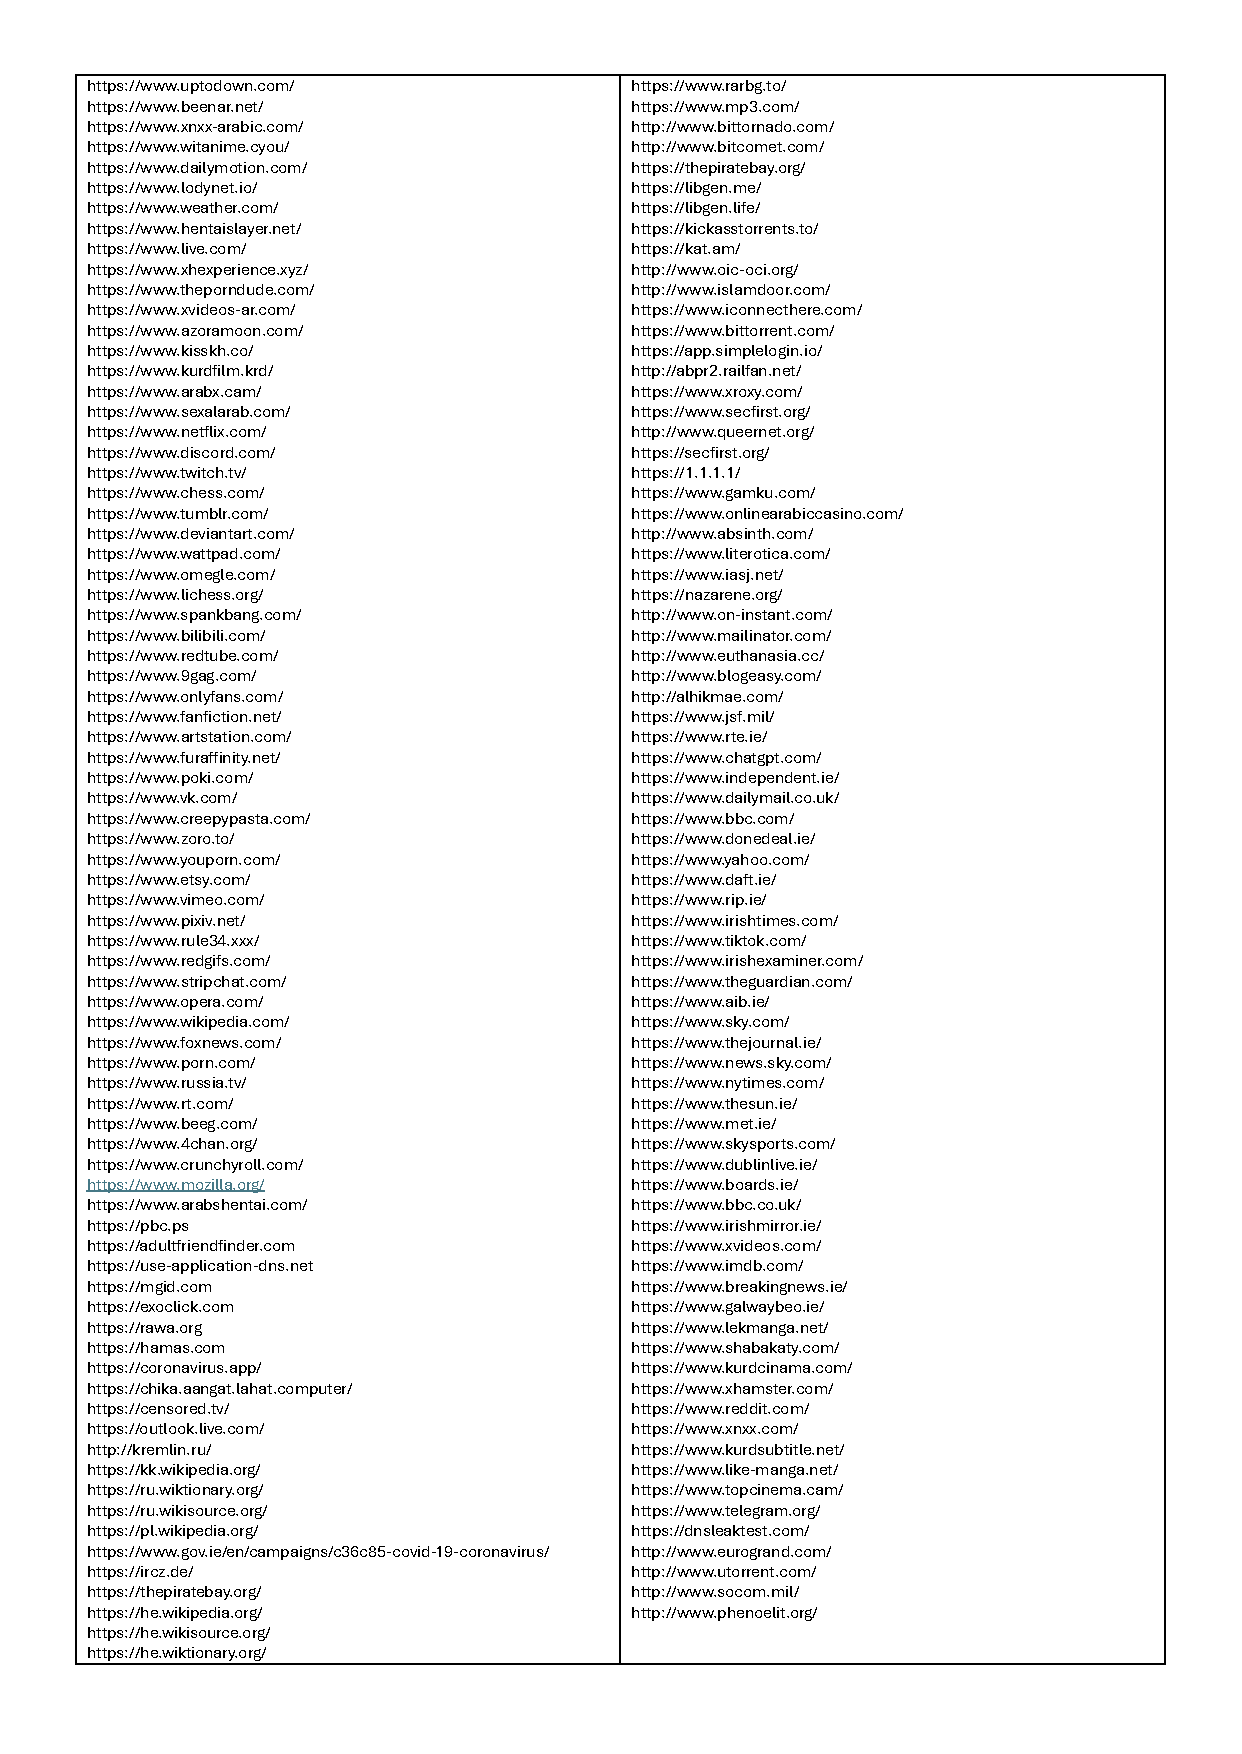
\includegraphics[width=1\linewidth]{appendix/my-webs1.pdf}
    \caption{my-websites.txt contains my curated list of sensitive domains}
    \label{fig:enter-label}
\end{figure}

\subsection{my-websites Results: Ireland}

\begin{tabular}{ll} 
\toprule
\textbf{Blocking Method} & \textbf{Websites} \\
\midrule
TCP/IP & \url{http://www.socom.mil} \\
       & \url{https://www.mp3.com} \\
       & \url{http://www.bittornado.com} \\
       & \url{https://libgen.life} \\
       & \url{http://www.oic-oci.org} \\
       & \url{https://doh.centraleu.pi-dns.com/dns-query?...} \\
       & \url{https://im0-tub-com.yandex.net/...} \\
       & \url{https://www.xroxy.com} \\
       & \url{http://www.queernet.org} \\
       & \url{https://www.gamku.com} \\
       & \url{https://www.onlinearabiccasino.com} \\
       & \url{https://www.iasj.net} \\
       & \url{https://www.shabakaty.com} \\
       & \url{http://alhikmae.com} \\
\midrule
DNS    & \url{https://thepiratebay.org} \\
       & \url{https://kickasstorrents.to} \\
       & \url{https://www.iconnecthere.com} \\
       & \url{https://www.rt.com} \\
\midrule
HTTP   & \url{http://www.euthanasia.cc} \\
\bottomrule
\end{tabular}

\vspace{1cm}

\subsection{my-websites Results: Israel}

\begin{tabular}{ll}
\toprule
\textbf{Blocking Method} & \textbf{Websites} \\
\midrule
TCP/IP & \url{http://www.socom.mil} \\
       & \url{https://www.mp3.com} \\
       & \url{http://www.bittornado.com} \\
       & \url{https://libgen.life} \\
       & \url{http://www.oic-oci.org} \\
       & \url{https://doh.centraleu.pi-dns.com/dns-query?dns=q80BAAABAAAAAAAAA3d3dwdleGFtcGxlA2NvbQAAAQAB} \\
       & \url{https://im0-tub-com.yandex.net/i?id=462f375c96139f1e41d919b44be2d780\&n=13\&exp=1} \\
       & \url{https://www.xroxy.com} \\
       & \url{http://www.queernet.org} \\
       & \url{https://www.onlinearabiccasino.com} \\
       & \url{https://www.iasj.net} \\
       & \url{http://alhikmae.com} \\
       & \url{https://www.shabakaty.com} \\
\midrule
DNS    & \url{https://www.gamku.com} \\
\midrule
HTTP   & \url{http://www.euthanasia.cc} \\
\bottomrule
\end{tabular}





\end{document}